\documentclass[grad,pdftex,numbers]{coppetex/coppe}
\usepackage[utf8]{inputenc}
\usepackage{amsmath,amssymb}
\usepackage{lmodern}
\usepackage{float}
\usepackage{multirow}
\usepackage{subfigure}
\usepackage{listings}
\usepackage{longtable}
\usepackage{placeins}

% Configure listings package
\lstset{ %
language=Java,                % choose the language of the code
basicstyle=\footnotesize\sf,    % the size of the fonts that are used for the code
numbers=left,                   % where to put the line-numbers
numberstyle=\footnotesize,      % the size of the fonts that are used for the line-numbers
stepnumber=1,                   % the step between two line-numbers. If it's 1 each line 
                                % will be numbered
numbersep=5pt,                  % how far the line-numbers are from the code
showspaces=false,               % show spaces adding particular underscores
showstringspaces=false,         % underline spaces within strings
showtabs=false,                 % show tabs within strings adding particular underscores
frame=single,                   % adds a frame around the code
tabsize=4,                      % sets default tabsize to 4 spaces
captionpos=t,                   % sets the caption-position to top
breaklines=true,                % sets automatic line breaking
breakatwhitespace=true,         % sets if automatic breaks should only happen at whitespace
title=\lstname,                 % show the filename of files included with \lstinputlisting;
                                % also try caption instead of title
escapeinside={\%*}{*)},         % if you want to add a comment within your code
morekeywords={}                 % if you want to add more keywords to the set
}
\renewcommand{\lstlistingname}{Arquivo}

\makeloabbreviations

\begin{document}
  \title{Desenvolvimento Ágil e Modelo de Negócios voltados para Aplicações Web}
  \foreigntitle{Agile Development and Business Model for Web Applications}
  \author{Ariel}{Schvartz}
  \sauthor{Leonardo Gardel}{Valverde}
  \advisor{Prof.}{José Ferreira}{de Rezende}{Dr.}


  \examiner{Prof.}{José Ferreira de Rezende}{Dr.}
  \examiner{Prof.}{Aloysio de Castro Pinto Pedroza}{Dr.}
  \examiner{Prof.}{Jorge Lopes de Souza Leão}{Dr. Ing.}

  \department{PEE}
  \date{09}{2013}

  \keyword{Sistemas Web}
  \keyword{Ruby on Rails}
  \keyword{MVC}
  \keyword{TDD}
  \keyword{RESTful}

  \foreignkeyword{Web Systems}
  \foreignkeyword{Ruby on Rails}
  \foreignkeyword{MVC}
  \foreignkeyword{TDD}
  \foreignkeyword{RESTful}


  \maketitle

  \frontmatter
  \chapter*{Agradecimentos}

\begin{itemize}
\item Por Ariel Schvartz

Agradeço à toda minha família, principalmente meus pais que sempre estiveram presentes e me apoiaram em todos os momentos, tanto bons quanto ruins. Agradeço especialmente ao meu avô que hoje não está mais aqui, porém estaria muito feliz de estar vivendo esse momento ao meu lado. Agradeço a todos os meus amigos e à minha namorada, que me trazem ânimo e felicidade todos os dias. Por fim, agradeço ao Leo, parceiro no trabalho final que certamente será um parceiro para toda a vida.

\item Por Leonardo Gardel Valverde

Agradeço à minha mãe, que sempre esteve presente física e mentalmente em todos os momentos importantes da minha vida. Agradeço ao meu pai e minha irmã, que, apesar do recente distanciamento, me ensinaram muito e encheram meus dias de lembranças e saudade. Agradeço aos meus amigos, que fazem a vida valer a pena. Por fim, agradeço ao meu amigo e companheiro de projeto, Ariel, por sua excelente companhia e seu grande empenho em fazer tudo dar certo.

\item Por Ambos

Agradecemos ao nosso orientador, que é um exemplo como profissional e como pessoa, dedicado e companheiro.

\end{itemize}

  \begin{abstract}

O sucesso e rentabilidade de diversos sistemas web instigam o surgimento de novos empreendimentos na área de computação. Porém, é importante saber como fazê-lo diante de uma infinidade de alternativas para o desenvolvimento e planejamento de tais aplicações por suas equipes. Este trabalho visa orientar tais empreendimentos, apresentando conceitos e métodos, que além de modernos, são frequentemente requisitados no mercado de software atual para o desenvolvimento ágil. Por fim, será apresentada uma implementação onde tais conceitos são aplicados, além de um modelo de negócios do projeto.

\end{abstract}
  \begin{foreignabstract}

The success and profitability of many web systems instigates the emergence of new ventures in computing. However, it is important to know how to do it, in front of a plethora of alternatives for the development and planning of such applications by their teams. This work aims to guide these ventures, presenting modern concepts and methods that are often required in the software market today for agile development. Lastly, will be presented an implementation where this concepts are applied, aside from a project business model.

\end{foreignabstract}


  \tableofcontents
  \listoffigures
  \listoftables
  \printloabbreviations

  \mainmatter
  \chapter{Introdução}

O protocolo HTTP (Hypertext Transfer Protocol),
\abbrev{HTTP}{Hypertext Transfer Protocol}
além de linguagens como o HTML (HyperText Markup Language),
\abbrev{HTML}{HyperText Markup Language}
permitiram o surgimento dos primeiros navegadores web, marcando o início da chamada Web 1.0. Nesta primeira versão, que vigorou ao longo dos anos 90, seu objetivo era simplesmente prover informação, já que o conteúdo presente em sua maioria era do tipo ``somente leitura''~\cite{slidesweb}.

Surge então a Web 2.0, por volta de 1999, onde o conteúdo da rede passa a ser largamente preenchido pelos usuários, através de blogs ou redes sociais, por exemplo~\cite{videoweb}. Desde então, aplicações web extremamente rentáveis (como o Facebook, que registrou um lucro líquido no segundo trimestre de 2013 de cerca de 333 milhões de dólares~\cite{facebooklucro}) instigam o surgimento de novos empreendimentos. Isso aliado com a crescente difusão dos conhecimentos necessários ao desenvolvimento de aplicações web, tornou o mercado extremamente competitivo. Tal competitividade torna a agilidade característica essencial aos novos empreendedores, na implantação e manutenção de seus negócios.

\section{Motivação}

Para os novos empreendimentos em computação, não faltam oportunidades ou ideias, especialmente no ambiente universitário.  Esta área é extremamente favorável a criação destes, pois as possibilidades para a inovação são inúmeras, além do baixo capital inicial demandado por tais iniciativas.

Entretanto, para que consigamos colocar muitas ideias em prática, além de garantir que cada ideia seja desenvolvida em pouco tempo (essencial para garantir competitividade no mercado), os esforços no desenvolvimento das mesmas devem ser reduzidos. Para isso, é extremamente interessante que se utilize um bom \textit{framework} de desenvolvimento.

Utilizar um \textit{framework} é simplesmente reutilizar código desenvolvido por terceiros, porém existe uma grande diferença entre este e as chamadas bibliotecas. Uma biblioteca é utilizada para uma função específica, complementando o fluxo de controle da sua aplicação, ao passo que os \textit{frameworks} definem este fluxo, mas permitem personalização para se atingir a funcionalidade desejada. Trata-se da chamada inversão de controle. Sendo assim, o uso de \textit{frameworks} é muito interessante para sistemas web, uma vez que o fluxo de controle destes em geral é igual ou muito semelhante~\cite{wikipediaframework}.

Para que possamos entender melhor os \textit{frameworks} para sistemas web, vamos focar em suas atividades mais gerais. A grande maioria de seus fluxos se baseia, respectivamente, na recepção de requisições HTTP, no acesso ao BD (banco de dados),
\abbrev{BD}{banco de dados}
no tratamento dos dados recebidos pelas requisições ou pelo BD e na resposta ao usuário através de uma página HTML pertinente. Sendo assim, é interessante tornar genérica essa lógica de controle, evitando o retrabalho dos desenvolvedores. Uma vez que a ``espinha dorsal'' do sistema já está a cargo do \textit{framework}, todo o esforço de implementação fica diretamente relacionado às especificidades do projeto.

Entretanto, a tarefa de escolher um \textit{framework} não é trivial, diante das inúmeras possibilidades existentes. Podemos optar pelo \textit{framework} somente com base nas linguagens a serem utilizadas, mas, a longo prazo, dificilmente esse critério resultará melhor escolha. Para fazer uma boa escolha, é interessante saber as características desejáveis em um \textit{framework} para sistemas web. É interessante que este possua:~\cite{frameworkexplain}
\begin{itemize}
\item uma abstração interessante como interface com o BD

O código escrito na aplicação não deve ser específico para o BD a ser utilizado. Isso requer uma interface de acesso ao mesmo que abstraia as suas especificidades, permitindo que um mesmo código seja utilizado para acesso a diversos tipos de bancos de dados. Também é muito interessante a utilização de ORM (Object-relational mapping)
\abbrev{ORM}{Object-relational mapping}
para tornar mais amigável o manuseio de dados do BD. Além disso também é importante que o \textit{framework} permita a validação dos dados a serem persistidos de forma manutenível.

\item ferramentas facilitadoras para a construção de páginas web

É interessante que o \textit{framework} facilite a criação de páginas web, de forma que seja necessário pouco ou nenhum entendimento sobre linguagens como HTML ou CSS (Cascading Style Sheets).
\abbrev{CSS}{Cascading Style Sheets}
Para isso, devem ser fornecidas funções que automatizem a criação do código de estilo.

\item um sistema eficaz de autenticação

Diversos sites permitem aos usuários o acesso de forma anônima, mas boa parte deles requer autenticação. Por ser uma necessidade comum a muitos sistemas, deve ser oferecida pelo \textit{framework} de forma opcional. Dentro deste tópico estão incluídas diversas funcionalidades, como a criação de contas, recuperação das mesmas, abertura de sessão, entre outras.

\item segurança

Autenticação e autorização andam sempre lado a lado. Após autenticado, é necessário ter o controle sobre as operações (como leitura ou escrita) realizadas pelos usuários. O conjunto formado por usuário, informação e operação deve ser autorizado antes da ação ser executada. Uma falha de segurança pode ser, por exemplo, permitir que um usuário altere dados de algum outro, ou que acesse dados confidenciais.

\item eficiência

As operações realizadas pelo \textit{framework} devem ser otimizadas, especialmente no acesso aos dados do BD e no carregamento das páginas web, visando um menor tempo total de resposta do servidor. Uma das maneiras de alcançar este objetivo é permitir que os dados sejam armazenados em cache.

\item método simples para criação e utilização de bibliotecas

Para o desenvolvimento ágil, é essencial a reutilização de código. Sendo assim, é importante que a inclusão ou criação de bibliotecas não seja uma operação custosa.

\item uma grande comunidade que o utiliza

Quanto mais pessoas utilizando o \textit{framework}, melhor. Isso faz com que as bibliotecas sejam melhor revisadas e, consequentemente, atualizadas. Além disso, a busca por informação é facilitada, uma vez que a quantidade de informação disponível a respeito de um \textit{framework}, em geral, é proporcional ao tamanho da sua comunidade.

\end{itemize}

É importante não se ater apenas às questões relativas à implementação. Um empreendimento perfeitamente implementado, porém com baixa aceitação por seu público ou pouco rentável, representa apenas tempo e dinheiro perdidos. Para que isso não aconteça, é necessário avaliar o seu empreendimento enquanto negócio, preferencialmente antes mesmo de ser escrita a primeira linha de código.

\section{Objetivo}

O objetivo deste trabalho é apresentar um método moderno e ágil para planejamento e implementação de sistemas web. Entretanto, não terá um cunho puramente teórico. A partir de uma ideia, detalhada na próxima seção, será realizada a implementação (apresentada no capítulo 3) e o planejamento do negócio (apresentado no capítulo 4), até que um protótipo seja desenvolvido.

\section{A ideia}

Dado que será implementada uma aplicação web real, que seja algo interessante e possivelmente rentável, sendo assim passível de planejamento enquanto negócio. Observando alguns dos aplicativos web existentes para a gerência de eventos, isto é, aqueles que auxiliam os seus usuários a administrar e planejar de forma organizada eventos (como shows, festas, entre outros), é possível notar que nenhum possui todas as funcionalidades demandadas por seus usuários, obrigando-os a recorrer a sistemas complementares. Surgiu então a ideia de criar uma plataforma que auxilie de forma plena seus usuários nesse tipo de demanda.

Para avaliar como e porque não existe uma plataforma completa com esta finalidade, vamos refletir sobre os tipos de eventos possíveis. Sabemos que, quanto à privacidade, os eventos podem ser abertos (públicos) ou fechados (privados), porém, quanto ao pagamento, um evento pode ser:
\begin{itemize}
\item fixo, onde são vendidos ingressos a preços predefinidos (ou gratuito)

Esses eventos são implementados em diversos aplicativos web, como o Facebook, Lista Amiga ou Eventick, porém os dois primeiros não possuem uma funcionalidade de pagamento. Neste caso, em geral os usuários informam que o pagamento deve ser realizado através de outros sites, como o Ingresso Rápido ou o Ingresso Certo. O Eventick implementa um sistema de pagamento e possui integração com redes sociais, no entanto os usuários não podem ser convidados para um evento, eles precisam se inscrever voluntariamente para fazer parte dos mesmos.

\item compartilhado, onde o custo total é dividido igualmente entre os convidados

Existem alguns aplicativos simples e que dão suporte a esse tipo de eventos, porém funcionam apenas localmente, como calculadoras.

\item colaborativo, onde ocorre a divisão de responsabilidades sobre itens

Neste tipo de evento, o organizador define uma lista de itens a serem levados, com suas respectivas quantidades. Cada participante se responsabiliza por levar um ou mais itens no dia do evento. É importante que o valor total dos itens a serem levados por cada participante seja aproximadamente igual.

Seria interessante uma ferramenta que auxiliasse neste tipo de evento por ser de difícil gerenciamento, mas não é implementado por nenhum aplicativo conhecido.

\end{itemize}

Além de permitir a criação e acesso à eventos, é interessante que se possa buscar por eventos de forma eficiente. Diversos algoritmos de busca podem ser implementados para realizar um bom ranqueamento dos eventos. Esses algoritmos podem ser baseados em relacionamentos (como o Facebook), em popularidade (como o Lista Amiga) ou ate por geolocalização.

Nossa ideia é reunir a interação social do Facebook, o bom ranqueamento do Lista Amiga e o sistema de pagamento do Eventick, para construir um sistema único e auto suficiente. Serão implementadas também outras funcionalidades como: eventos colaborativos, eventos compartilhados, notificações por e-mail, entre outros.

\section{Estruturação do documento}

No capítulo 2, veremos as metodologias utilizadas no desenvolvimento do \textit{software} e os motivos de sua utilização. Em seguida, o capítulo 3 detalha a implementação através das metodologias elucidadas. O capítulo 4 apresenta o modelo de negócios desenvolvido, enquanto o capítulo 5 visa concluír o trabalho e apontar melhorias necessárias em trabalhos futuros.
  \chapter{Ferramentas e Metodologias Utilizadas}

Obviamente, assim como todas as outras aplicações web, foi utilizado o protocolo HTTP para comunicação entre cliente e servidor. Essa comunicação se inicia quando o cliente (no caso, o navegador do usuário) realiza uma requisição HTTP. Ao receber a requisição, o servidor web a processa, gera uma resposta pertinente e a devolve ao cliente~\cite{wikipediahttp}.

O código de aplicações web é dividido em duas principais categorias: o \textit{frontend}, responsável pela interação com o usuário, e o \textit{backend}, responsável por todo o processamento realizado no servidor. A compreensão desta distinção é essencial, pois existem linguagens e metodologias específicas, tanto para o desenvolvimento de cada uma delas, como para o planejamento da comunicação entre esses dois mundos. Mais adiante, as duas categorias serão explicadas em mais detalhes.

\section{RESTful}

O protocolo HTTP foi desenvolvido em paralelo com a arquitetura REST (Representational State Transfer),
\abbrev{REST}{Representational State Transfer}
que serve de molde para o desenvolvimento de aplicativos web, pois ilustra como eles devem se comportar~\cite{restthesis}. Uma aplicação que é desenvolvida segundo a arquitetura REST, é dita RESTful. Seguindo esta arquitetura no desenvolvimento da aplicação, uma série de vantagens são obtidas, como uma melhora na escalabilidade da mesma. Isto ocorre pois esta arquitetura segue uma lógica \textit{stateless}, isto é, o servidor não armazena estados, sendo necessária a transmissão de todas as informações inerentes ao processamento das requisições por meio das mesmas.

Para que a aplicação seja RESTful, devemos nos preocupar com alguns detalhes. É importante que cada recurso seja representado por uma única URI (Uniform Resource Identifier),
\abbrev{URI}{Uniform Resource Identifier}
mas para que isso seja possível, é necessário explorar ao máximo os seus métodos. Como a maioria dos recursos precisam ser relacionados a cada uma das ações do CRUD (Create, Retrive, Update, Destroy),
\abbrev{CRUD}{Create, Retrive, Update, Destroy}
é interessante que tais ações sejam relacionadas diretamente com os métodos do protocolo HTTP, visando manter inviolável a relação entre a URI e o recurso. Sendo assim, os quatro principais métodos do protocolo HTTP, que serão invocados no \textit{frontend}, devem ser relacionados aos quatro métodos do CRUD, que serão invocados no \textit{backend}. Em geral essa relação ocorre da seguinte forma:
\begin{itemize}
\item C (Create) - método POST
\item R (Retrive) - método GET
\item U (Update) - método PUT
\item D (Destroy) - método DELETE
\end{itemize}

\section{\textit{Frontend}}

O \textit{frontend} da aplicação é todo o código encarregado de realizar a interação com o usuário. No caso, trata-se de tudo que será enviado ao navegador. Esse código tem a finalidade de exibir de forma inteligível e interessante o resultado da requisição tratada pelo \textit{backend}, além de lidar com as entradas de dados (\textit{inputs}) do usuário. Para a construção do \textit{frontend} utilizamos algumas linguagens e bibliotecas, que serão elucidadas a seguir.

\subsection{HTML}

O HTML é a linguagem base do \textit{frontend}, pois as demais operam sobre seus elementos. Ela torna possível a interpretação das páginas web pelos navegadores. Esta linguagem sofreu algumas atualizações, porém, após mais de dez anos sem novas versões, ficou bastante defasada. Com os avanços da Internet, passaram a ser utilizados inúmeros \textit{plug-ins} para que páginas web fossem capazes de realizar algumas atividades essenciais, como reprodução de vídeos ou de áudio.

Esse atraso se prolongou até 2008, quando foi publicada uma nova versão, o HTML5, que ainda não esta completamente em vigor, porém cada vez mais em uso~\cite{wikipediahtml}. Essa nova versão dá suporte a diversas funcionalidades sem que sejam necessários \textit{plug-ins}. Dentre as funcionalidades implementadas estão a reprodução de vídeos , áudios, o \textit{drag and drop} e a exibição de imagens vetorizadas~\cite{videohtml}.

\subsection{CSS}

O CSS é uma linguagem criada para estilização de componentes HTML. Podemos dizer que os navegadores interpretam o CSS como adjetivos dos componentes HTML. É uma linguagem voltada para o ``como exibir'', enquanto o HTML se preocupa com ``o que exibir''. O CSS3, sua versão mais recente que trouxe diversas novas funcionalidades, vem sendo cada vez mais utilizado.

\subsection{Javascript}

O Javascript é uma linguagem de programação que, apesar de ser utilizada no desenvolvimento do \textit{frontend} da aplicação, se assemelha às linguagens de \textit{backend}, pela liberdade oferecida ao programador. É utilizada para dar interatividade às páginas web, visto que, apesar de essenciais, o HTML e o CSS não fornecem muita dinamicidade à mesma. Através da utilização de Javascript é possível alterar de forma livre o conjunto composto pelo HTML e CSS, mesmo após o carregamento completo da página. Inúmeras bibliotecas são construídas através da linguagem Javascript. Muitas delas também são utilizadas no \textit{frontend} de aplicações web, como a JQuery.

\subsection{AJAX (Asynchronous JavaScript and XML)}
\abbrev{AJAX}{Asynchronous JavaScript and XML}

O AJAX é um conjunto de técnicas que permite a criação de requisições assíncronas em páginas web. A sua utilização é interessante quando é necessária a troca de dados sem que seja preciso recarregar a página por inteiro. Resumidamente, uma implementação de AJAX é um trecho de código em Javascript, que faz com que seja realizada uma requisição XHR (XML HTTP Request),
\abbrev{XHR}{XML HTTP Request}
que será tratada e respondida pelo servidor. Essa resposta, que em geral é no formato XML (Extensible Markup Language)
\abbrev{XML}{Extensible Markup Language}
ou JSON (JavaScript Object Notation),
\abbrev{JSON}{JavaScript Object Notation}
é recebida pelo Javascript, podendo ser utilizada para atualizar elementos.

\subsection{JQuery}

A JQuery é talvez a biblioteca mais utilizada em Javascript no desenvolvimento de aplicações web. Diversas funcionalidades interessantes são implementadas por esta biblioteca, dentre elas, uma interface amigável para customização de requisições AJAX. É muito utilizada também para criar animações, como a inserção de elementos na tela de forma gradual.

\section{\textit{Backend}}

O \textit{backend} da aplicação é todo o código responsável pelo processamento da requisição até o momento da geração da resposta. Para exemplificar, pode-se pensar em uma requisição de abertura de sessão (\textit{login}) por meio da aplicação. Neste caso, o \textit{backend} é o código responsável por atividades como a verificação da existência do usuário ou a validação da senha inserida pelo mesmo. O \textit{backend} determina também qual o tipo da resposta que será devolvida ao usuário (falha ou sucesso na abertura de sessão, segundo o exemplo). Observando por outro prisma, o \textit{backend} pode ser encarado como o código responsável pela tomada de decisão.

O \textit{backend} pode ser implementado em inúmeras linguagens. Como é muito comum e recomendada a utilização de \textit{frameworks}, as linguagens relativas a estes acabam sendo as mais utilizadas. Linguagens como o SQL também são utilizadas no \textit{backend} da aplicação, já que o BD também o compõe.

Existem diversos \textit{frameworks} nas mais variadas linguagens, porém o escolhido para este trabalho foi o Ruby on Rails. A seguir serão explicados com detalhes os motivos da escolha, através de funcionalidades deste \textit{framework}.

\section{A escolha do Ruby on Rails}

O desenvolvimento ágil de aplicações web teve início com o surgimento do Ruby on Rails. Esta agilidade na implementação se deve a uma série de princípios adotados no desenvolvimento deste \textit{framework}, como o DRY (Don't Repeat Yourself) e o CoC (Convention over Configuration)~\cite{ieeecomparsionagileframeworks}. O DRY é um princípio de desenvolvimento de software que introduz a ideia de que uma mesma informação não deve ser repetida mais de uma vez ao longo do código. Este princípio simplifica o trabalho do desenvolvedor, evitando redundâncias e os problemas causados por elas. O CoC implica em adotar por padrão uma mesma configuração. Caso o desenvolvedor queira fugir do padrão, deve escrever código para isso, porém não deve escrever uma única linha para seguir os padrões.

Por ser pioneiro em desenvolvimento ágil de aplicações web, o Ruby on Rails teve o seu grande momento logo após o seu lançamento, e, por volta de 2006, atingiu o seu pico de interesse. Até hoje existe uma grande comunidade que o utiliza, porém, após o surgimento de diversos outros \textit{frameworks} para desenvolvimento ágil, ocorreu significativa queda no interesse. Estabilizou-se então dentre os \textit{frameworks} mais utilizados, como podemos notar através da figura~\ref{fig:curvainteresserails}, que indica a curva de interesse sobre os \textit{frameworks} ao longo dos anos.

\begin{figure}[H]
\centering
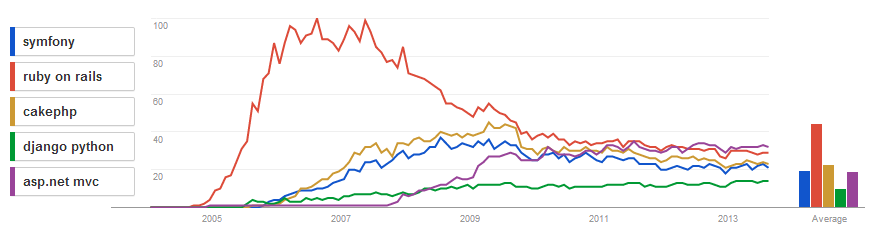
\includegraphics[width=0.8\textwidth]{figs/curva_de_interesse}
\caption[\textit{Curva de Interesse sobre os \textit{frameworks} ao longo dos anos}.]
{Curva de Interesse sobre os \textit{frameworks} ao longo dos anos~\cite{curvadeinteresseframeworks}.}
\label{fig:curvainteresserails}
\end{figure}

O Ruby on Rails é um \textit{framework} dito \textit{full-stack}, por ser utilizado obrigatoriamente por inteiro (ao contrário de outros \textit{frameworks}, onde seus módulos podem ser utilizados separadamente, como o Zend). Possui uma arquitetura MVC (Model-View-Controller),
\abbrev{MVC}{Model-View-Controller}
muito comum em diversos \textit{frameworks}, que será melhor detalhada a seguir. Esta arquitetura aplicada em um \textit{framework} \textit{full-stack} e aliada a conceitos como o DRY e o CoC, permite que em pouquíssimas linhas de código, enormes funcionalidades sejam implementadas, como veremos mais a frente.

\subsection{Arquitetura MVC}

Esta arquitetura realiza uma separação entre a parte que interage com o usuário (a visão) e a informação (o modelo), permitindo que esta seja acessada por meio de métodos em classes específicas (os controladores). Esta forma modularizada de desenvolvimento provê um excelente isolamento entre essas camadas com funções tão distintas, viabilizando a reutilização de código e tornando o mesmo mais legível, e, consequentemente, manutenível.

A figura ~\ref{fig:mvc} apresenta a arquitetura MVC aplicada ao \textit{framework} Ruby on Rails~\cite{basefiguramvc}. O servidor web repassa as requisições recebidas a um sistema de rotas, que é encarregado de enviá-las ao controlador correspondente. O sistema de rotas muitas vezes é definido no próprio servidor web, porém, o Rails possui sistema de rotas independente, como será elucidado na subseção ~\ref{subsec:sistrotas}. Os demais componentes, relativos ao MVC, serão melhor detalhados a seguir.

\begin{figure}[H]
\centering
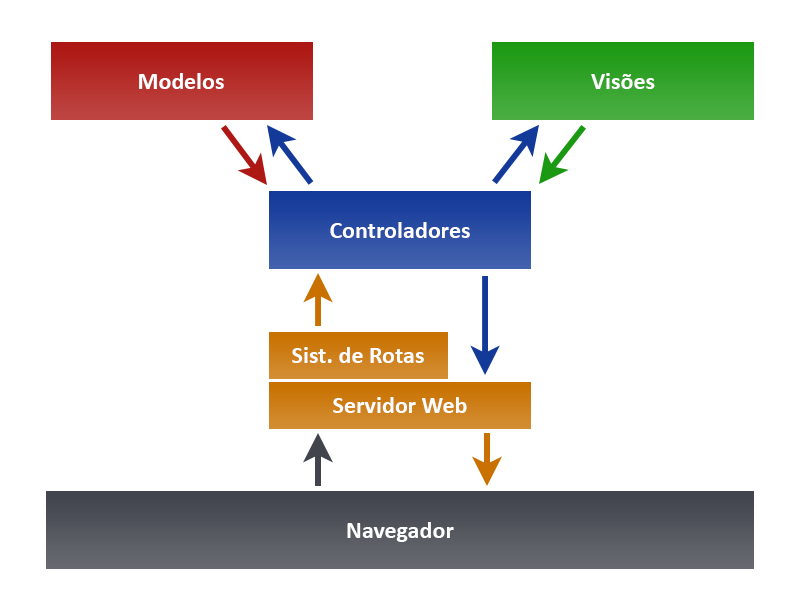
\includegraphics[width=0.8\textwidth]{figs/mvc}
\caption[\textit{Arquitetura MVC do \textit{framework} Ruby on Rails}.]
{Arquitetura MVC do \textit{framework} Ruby on Rails.}
\label{fig:mvc}
\end{figure}

\begin{itemize}

\item O Modelo

O modelo é o módulo responsável pela gerência do conhecimento da aplicação e sua manipulação segundo métodos específicos. Em geral, as aplicações utilizam BD, porém existem exemplos de aplicações em que não é interessante o seu uso. No primeiro caso, os modelos em geral estabelecem uma relação de um para um com as estruturas de objetos (as tabelas do BD). Códigos especialistas, como buscas eficientes em BD ou manipulação e validação de dados inseridos pelos usuários, devem ser pertencentes aos modelos.

\item A Visão

A visão é, em geral, a representação visual do seu modelo. Todo o código do \textit{frontend} da aplicação é parte das visões. Comumente são utilizadas linguagens para mesclar dados variáveis (resultado das requisições) com as visões, além de fazer o chamado \textit{templating}, que será melhor elucidado ainda neste capítulo. No Ruby on Rails, são utilizadas linguagens como o ERB (Embedded Ruby)
\abbrev{ERB}{Embedded Ruby}
e o Haml (HTML Abstraction Markup Language)
\abbrev{Haml}{HTML Abstraction Markup Language}
para esta finalidade.

\item O Controlador

O controlador é responsável por conectar os usuários ao sistema em si. Informações presentes nas requisições HTTP realizadas e informações extraídas dos modelos, servem de base para os controladores, que, segundo uma lógica definida pelo implementador, definem o fluxo resultante da requisição.

\end{itemize}

Para exemplificar o funcionamento geral dos módulos elucidados, será utilizado novamente o caso do usuário que tenta realizar uma abertura de sessão. Quando a requisição HTTP é disparada, por meio do mecanismo de rotas (que será detalhado mais a frente), esta requisição chega a um controlador. Este, por sua vez, acessa o modelo e verifica a validade dos dados, como a existência do usuário e a corretude da senha inserida. O controlador decide então por abrir a sessão do usuário e redirecioná-lo para a visão correspondente ou por recarregar a página de tentativa de abertura de sessão, exibindo uma mensagem de erro pertinente.

\subsection{Sistema de rotas independente}
\label{subsec:sistrotas}

Uma aplicação em Rails implementa o seu próprio sistema de rotas, que é independente do servidor web que está sendo utilizado. O servidor padrão oferecido é o WEBrick, em Ruby, porém outros servidores podem ser utilizados sem que o esquema de rotas precise ser alterado. Trata-se de um arquivo onde, basicamente, é feita a correspondência entre os controladores e o conjunto de recursos e métodos das requisições HTTP.

\subsection{Incentivo à programação RESTful}

Além dos princípios citados, o Ruby on Rails incentiva a programação RESTful através de algumas de suas configurações padrão. Para a criação de rotas RESTful em sua aplicação, basta apenas uma linha de código. Esta linha define que deve ser gerada a correlação entre o CRUD de um recurso e os métodos HTTP sobre uma URI referente ao recurso. Para ser mais claro, essa única linha de código resulta na criação de rotas como indica a tabela~\ref{table:tabautorotas}.

\begin{center}
\begin{longtable}{|c|c|c|}

\caption[Tabela de rotas automáticas para recursos no Ruby on Rails.]
{Tabela de rotas automáticas para recursos no Ruby on Rails}
\label{table:tabautorotas} \\

\hline \multicolumn{1}{|c|}{\textbf{Método HTTP}} & \multicolumn{1}{c|}{\textbf{Endereço}} & \multicolumn{1}{c|}{\textbf{Ação}} \\ \hline 
\endfirsthead

\multicolumn{3}{c}%
{{\bfseries \tablename\ \thetable{} -- continuação}} \\
\hline 
\multicolumn{1}{|c|}{\textbf{Método HTTP}} &
\multicolumn{1}{c|}{\textbf{Endereço}} &
\multicolumn{1}{c|}{\textbf{Ação}} \\ \hline 
\endhead

\endfoot

\hline
\endlastfoot

GET & /usuarios & index \\
GET & /usuarios/new & new \\
POST & /usuarios & create \\
GET & /usuarios/:id & show \\
GET & /usuarios/:id/edit & edit \\
PUT & /usuarios/:id & update \\
DELETE & /usuarios/:id & destroy \\

\end{longtable}
\end{center}

Com exceção do método \textit{show} (que é equivalente ao método \textit{retrieve} no CRUD), os outros três métodos do CRUD possuem nomes equivalentes. Entretanto, podemos notar que existem três métodos que não se encaixam no CRUD. Vamos analisar primeiramente o \textit{new} e o \textit{edit}. Eles foram criados visto que, para a realização de tarefas como \textit{update} ou \textit{create}, são necessários formulários, já que não é racional exigir que usuários comuns realizem manualmente requisições HTTP, fornecendo os parâmetros corretos para cadastro ou atualização. Por isso foram criados esses dois métodos, que exibem ao usuário páginas contendo formulários de cadastro e de atualização, viabilizando as operações de \textit{update} e de \textit{create}. Além destes foi criado o \textit{index}, que foi feito para dar lugar a uma página contendo (todos ou alguns) objetos equivalentes àquele recurso. Resumidamente, trata-se de um \textit{retrieve} em grupo.

\subsection{Geradores automáticos de código}

O Ruby on Rails possui outra característica interessante que provê agilidade no desenvolvimento: os geradores automáticos de código. Com um simples comando é possível evitar algum tempo de desenvolvimento utilizando esses geradores. Eles podem criar modelos, controladores, visões, migrações ao BD, ou até, todos ao mesmo tempo, como é o caso do gerador \textit{scaffold}.

Esta funcionalidade também é muito útil para instalação de bibliotecas externas (as chamadas gemas, como veremos a seguir). Muitas bibliotecas necessitam da criação de tabelas no BD para seu funcionamento pleno, ou oferecem visões prontas para seus primeiros usos. Desta forma, são criados instaladores automáticos para as bibliotecas, utilizando os geradores automáticos de código.

\subsection{Ferramentas de automatização de design de \textit{frontend}}

Ao programar em Rails, assim como em diversos outros \textit{frameworks} para desenvolvimento ágil, é possível implementar o design de suas visões de forma automatizada, ou resumida. Esta é uma importante tarefa dos \textit{frameworks}, pois faz com que seja necessário saber pouco ou nada sobre linguagens como CSS ou Javascript, para que seja desenvolvida uma página visualmente agradável. Apesar de o Rails não auxiliar na produção de estilos ou interatividade para a aplicação, como estes \textit{frameworks} de \textit{frontend}, ele fornece diversos recursos que facilitam enormemente a produção do conteúdo da aplicação (o código HTML).

Através das linguagens ERB e HAML, como dito anteriormente, é possível a utilização de operações em Ruby dentro dos arquivos de visões. Suponhamos que é necessário que a visão contenha 20 elementos HTML idênticos ou extremamente semelhantes. Esta tarefa seria extremamente penosa e repetitiva, além de produzir código redundante. Entretanto, com o Rails, é possível escrever um único elemento dentro de um iterador na linguagem Ruby, para obter o mesmo resultado. A linguagem HAML vai mais além. Sua utilização torna a produção de código mais legível e organizada, reduzindo boa parte do código inserido para produção de elementos HTML.

É comum que precisemos exibir os mesmos componentes em mais de uma visão da aplicação. Se tratando do \textit{framework} Ruby on Rails, um mesmo trecho de código replicado diversas vezes ao longo de toda a aplicação indica que é necessário um replanejamento do mesmo. Um iterador resolve o problema para o caso de código replicado em cadeia, porém existe uma boa solução para replicação de código de visões em geral: os parciais. Um parcial é um arquivo de visão auxiliar que pode ser invocado dentro de outras visões, ou até mesmo dentro de outros parciais. Ao invocar um parcial, o código de invocação é substituído pelo seu conteúdo. É possível que parciais recebam parâmetros no momento de sua invocação, possibilitando a personalização do resultado final em cada chamada.

Além disso, o Rails possui funções ajudantes (do inglês \textit{helpers}), que automatizam procedimentos que são comumente realizados pelos usuários. Enquanto os parciais auxiliam na criação de elementos de visão (em HTML), evitando a replicação de código, as funções ajudantes permitem que código Ruby seja inserido, com a mesma finalidade.

Outro mecanismo que dá praticidade à produção de código de visão são os \textit{templates}. Estes possibilitam que código seja adicionado sem que seja preciso sequer invocá-los. É muito comum a sua utilização quando é necessária a produção de um mesmo código de visão para diversas páginas, como em cabeçalhos. É comum que um aplicativo web possua diferentes estilos de cabeçalhos, como para usuários autenticados ou não autenticados. Apesar de serem distintos, estes cabeçalhos se repetirão ao longo de diversas visões. Neste caso é interessante que sejam incluídos em \textit{templates} que serão adotados pelos arquivos de visões.

\subsection{Ferramenta para envio de e-mails}

O Rails permite que, através do módulo \textit{Action Mailer}, sejam enviados e-mails com extrema praticidade pela aplicação. A formatação dos e-mails é realizada através dos \textit{mailers}, que são semelhantes aos controladores, e dos arquivos de visão relacionados. Os \textit{mailers} possuem funções que representam tipos diferentes de e-mails a serem enviados, cada um com seu respectivo arquivo de visão. Em cada função é definido o conteúdo dos campos que preenchem o e-mail, porém a descrição do mesmo é preenchida através do arquivo de visão, utilizando código HTML. Os e-mails podem possuir conteúdo dinâmico, assim como os demais arquivos de visão.

\subsection{A linguagem Ruby}

Ruby é a linguagem utilizada ao trabalhar com o \textit{framework} Ruby on Rails. Trata-se de uma linguagem totalmente orientada a objetos. Nela, até mesmo os números e classes são objetos. É extremamente dinâmica, permitindo inclusive que métodos sejam implementados em tempo de execução (é o chamado \textit{monkey patching})~\cite{eloquent_ruby}. Inspirada em linguagens como o SmallTalk, o Ruby é extremamente legível e manutenível, já que o código pode ser escrito sem operadores como parênteses ou colchetes (é o chamado \textit{poetry mode}, que funciona desde que não existam ambiguidades no código produzido). A implementação de código se aproxima cada vez mais da escrita livre de textos, abrindo mão de redundâncias e declarações desnecessárias, que representam grande parte dos caracteres escritos em grande parte das linguagens de programação. Novamente podemos observar que essa é uma característica que dá agilidade ao processo de desenvolvimento.

Outro ponto extremamente positivo do Ruby é a existência de um gerenciador de pacotes próprio, o RubyGems. Ele facilita de maneira excepcional a utilização de bibliotecas externas, aliado com os geradores automáticos de código. Em outras palavras, com duas linhas é possível incluir e instalar uma biblioteca para utilização. Com apenas mais uma linha é possível gerar (quando necessário) as modificações que configuram sua aplicação, de forma a se adequar à utilização da nova biblioteca. As bibliotecas são as chamadas gemas. Torna-se também trivial a atualização das versões instaladas das bibliotecas, sendo necessário apenas um comando para buscar atualizações e instalá-las.

\subsection{Boa abstração do BD}

Qualquer um que está habituado a armazenar dados em um BD sabe que não é uma tarefa fácil. Um dos motivos é a necessidade de se preocupar com sintaxe das consultas em SQL (linguagem dos bancos de dados relacionais) realizadas. É comum nos depararmos com operações que são normalmente interpretadas por um SGBD (Sistema de Gerência de Banco de Dados),
\abbrev{SGBD}{Sistema de Gerência de Banco de Dados}
mas que causam erros sintáticos em outros.

\subsubsection{O Active Record}

O Rails oferece por padrão uma biblioteca chamada ActiveRecord que possui uma série de módulos importantes que são, sem dúvida, uma das principais ferramentas do \textit{framework}. Esta biblioteca estabelece uma associação entre uma classe de modelo a uma tabela do BD. Com ela é possível lidar com os dados de forma muito mais amigável. Para executar consultas ao banco não é mais necessário ter o domínio da linguagem SQL, pois esta biblioteca cria uma abstração da interface com o BD, provendo uma outra interface muito mais amigável e em Ruby. Para que esta biblioteca consiga se relacionar corretamente com o banco, basta instalar a gema correspondente ao seu SGBD. Desta forma, o seu código não se altera ao se alternar entre os diferentes SGBDs.

O ActiveRecord simplifica também o acesso a objetos por meio de relacionamentos. Isso implica na realização de consultas automáticas utilizando a chave estrangeira pertencente a um objeto, permitindo o acesso de entidades relacionadas com a mesma facilidade de acesso dos atributos locais. Também é possível a utilização de transações para prover às operações propriedades como atomicidade, e, aliado com o sistema de travas (do inglês \textit{lock}), propriedades como isolamento e consistência.

\subsubsection{O Active Model}

Existe também uma outra biblioteca chamada ActiveModel que possui módulos essenciais para o desenvolvimento de aplicações de qualidade, que serão detalhados a seguir.

\subsubsection{Validação}

Com este módulo é possível garantir que os dados que serão persistidos no banco sejam válidos ou consistentes. Existe uma série de funções que automatizam os processos de validação mais comuns, como a \textit{validates\_presence\_of}, que garante que não sejam válidos registros onde os campos passados como parâmetro são nulos. Porém, é possível implementar suas próprias funções de validação, que podem ser exportadas para validadores externos às classes dos modelos, para que sejam reutilizadas em mais de um deles.

Tais validações ocorrem entre o instante em que o sistema requisita que um registro seja persistido no banco e o momento em que ele é persistido de fato. Caso a validação invalide o registro, é adicionado um erro ao registro (atraves do módulo de erros) e o mesmo não é persistido, garantindo a integridade do banco.

\subsubsection{Chamadas de Retorno}

É extremamente importante que possamos realizar ações em momentos oportunos, como após a atualização de determinado registro, ou antes do momento em que são realizadas as validações. Para isso foi criado o módulo das chamadas de retorno (do inglês \textit{callbacks}). Com estas chamadas é possível executar procedimentos em momentos específicos e muito oportunos.

Para exemplificar o uso deste módulo, pode-se imaginar que é necessário incrementar um contador em um registro do banco toda vez que ele for atualizado. Existe uma solução redundante e trabalhosa para isso, que exige que o implementador lembre de incrementar este contador em todos os locais do código onde o registro é atualizado Porém, é muito mais interessante realizar essa tarefa utilizando as chamadas de retorno. Para isso, basta implementar uma função no modelo que realize esse incremento, e passar essa função como parâmetro para o método \textit{before\_ save} do módulo de chamadas de retorno. Desta forma, função sempre será executada logo antes da atualização do registro. Note que, neste caso, a função só será invocada caso o registro passe por todas as validações.

\subsubsection{Observação}

O módulo de observação possibilita que sejam implementadas chamadas de retorno sobre uma classe, porém executadas fora da mesma. Na prática, criamos um observador que ``vigia'' uma ou mais classes de modelos, podendo executar chamadas de retorno sobre elas simultaneamente.

\subsubsection{Trapaça}

Outro módulo importante é o módulo de trapaça (do inglês \textit{dirty}). Pode ser aplicado para a seguinte situação: deseja-se incrementar o contador citado apenas para o caso de um determinado atributo ter sido alterado. Para isso, também há soluções análogas à explicada no exemplo das chamadas de retorno. Porém tais soluções não são escaláveis. Em conjunto com as chamadas de retorno, o módulo de trapaça pode ser utilizado para prover a solução ideal. Este módulo permite acessar informações sobre atributos alterados desde a sua última versão persistida em banco. O nome tão peculiar deste módulo se deve ao fato de que ele nos dá o poder de ``bisbilhotar'' as modificações realizadas e tomar decisões baseadas nelas.

\subsubsection{Nomeação}

Este módulo lida com a pluralização das palavras, uma vez que o \textit{framework} convenciona que, por exemplo, nomes de classes são no singular, porém suas tabelas correspondentes são nomeadas no plural. Isso torna o código mais legivel, porém pode causar problemas, principalmente em expressões que não são pluralizadas de forma regular. Para isso existe um arquivo de inflexões, onde devem ser informadas as pluralizações não regulares a serem utilizadas pelo sistema.

\subsubsection{Tradução}

Outro módulo semelhante é o de tradução, que se comunica com as ferramentas de internacionalização do sistema, elucidadas a mais a frente.

\subsubsection{Serialização}

Este módulo permite a transformação de registros de modelos em tabelas \textit{hash} serializáveis ou arquivos de texto plano, como XML ou JSON, para que possam ser exportados ou persistidos.

\subsection{Suporte à autenticação e autorização terceirizado}

O Rails por padrão não implementa sistemas de autenticação e autorização, porém existem gemas que desempenham estas funções com maestria, como veremos adiante. Apesar disso, existem sistemas que possibilitam a verificação de condições antes da realização das ações, são os chamados filtros.

Os filtros são uma funcionalidade que permite que em pouquíssimas linhas sejam realizadas verificações que, muitas vezes, estão ligados à autorização. Um exemplo disso são os \textit{before\_filters}, que muitas vezes são utilizados para avaliar se um usuário está autenticado ao sistema, antes de permitir a realização das ações correspondentes.

\subsection{Segurança}

Inúmeras questões referentes à segurança ficam a cargo do servidor web, como a prevenção contra ataques DDoS (Distributed Denial of Service)
\abbrev{DDoS}{Distributed Denial of Service}
por exemplo, porém, após o momento em que as requisições chegam ao sistema de rotas do Rails, é responsabilidade do \textit{framework} e do programador localizar todas as brechas do sistema. Esporadicamente são necessárias atualizações de segurança ao Ruby on Rails, porém a maioria esmagadora dos ataques bem sucedidos são ocasionados por descuido dos desenvolvedores da aplicação. O \textit{framework} divulga uma página alertando sobre falhas comuns e suas medidas preventivas~\cite{segurancarails}.

Uma destas medidas oferecidas pelo Rails é a utilização de conexões SSL (\textit{Secure Sockets Layer}).
\abbrev{SSL}{Secure Sockets Layer}
A aplicação pode ser configurada para exigir do usuário que seja estabelecida uma conexão SSL antes de permitir a utilização do sistema. Esta medida pode prevenir a chamada \textit{Session Hijacking}, que permite a um usuário atacante a utilização do sistema através de uma conta com sessão previamente iniciada e em atividade.

Ataques de injeção também são muito comuns em aplicações web. Elas podem ser de diversos tipos. Um dos mais utilizados é o XSS (Cross-Site Scripting),
\abbrev{XSS}{Cross-Site Scripting}
que é um ataque de injeção de textos capaz de prejudicar o usuário, seja simplesmente para tornar pior a sua experiência ao utilizar o sistema ou para fazer \textit{Session Hijacking}. É possível também fazer injeções a nível de BD, para outras finalidades. Caso o sistema não seja imune à injeção de dados de uma forma geral, as possibilidades são infinitas para os atacantes. Uma medida preventiva para ataques de injeção é filtrar os dados inseridos pelo usuário, sempre que necessário.

\subsection{Eficiente}

O Rails implementa duas funcionalidades que visam prover eficiência aos aplicativos: o \textit{Assets Pipeline} e o sistema de \textit{cache}.

\subsubsection{\textit{Assets Pipeline}}

O \textit{Assets Pipeline} é um módulo que auxilia na compilação de todos os arquivos que devem ser servidos ao navegador. Isto inclui os arquivos CSS, Javascript, fontes e imagens. Este módulo realiza atividades como:

\begin{itemize}
\item Concatenação de arquivos

Essa é uma característica muito importante, principalmente no ambiente de produção. Ela é capaz de reduzir o número de requisições necessárias para que o navegador seja capaz de exibir a página. Todos os arquivos CSS são concatenados em um único arquivo (também em CSS), chamado arquivo de manifesto. O mesmo ocorre para os arquivos Javascript, totalizando dois arquivos de manifesto. Para evitar que o navegador tenha que carregar estes dois arquivos sempre que ocorrerem novas requisições, o Rails utiliza uma estratégia de ``impressão digital''. Isso faz com que o navegador só requisite novamente os arquivos de manifesto que contenham impressões digitais diferentes das versões presentes em seu cache.

\item Compressão e minimização de arquivos

Esta atividade minimiza os arquivos CSS e Javascript. No caso dos arquivos CSS, todos os espaços e comentários são excluídos do arquivo. Em arquivos Javascript processos mais complexos são aplicados, porém foge ao escopo deste trabalho explicitá-los. Essas lógicas para minimização e compressão podem ser customizadas de forma a atender caso a caso da melhor forma possível.

\item Código de Alto Nível

O \textit{Assets Pipeline} permite a utilização de ERB dentro do código CSS ou Javascript, permitindo um mundo de possibilidades que antes não era possível. No momento de compilação, esse código é transformado de forma a gerar um arquivo simples CSS. Além disso, permite a utilização de linguagens que vêm sendo cada vez mais utilizadas, como Sass (uma linguagem de CSS que permite a utilização de variáveis e pseudo-funções) e CoffeeScript (uma forma de escrever Javascript com menos linhas de código).

\item Pré-compilação

A pré-compilação acelera muito a exibição da página. Ela permite que todo o código CSS e Javascript seja compilado apenas uma vez, para que seja servido repetidamente em todas as requisições recebidas. Por padrão, os arquivos de manifesto CSS e Javascript são pré-compilados, mas é fácil configurar para que outros arquivos também sejam.
\end{itemize}

\subsubsection{Cache}

Existem diversos níveis de cache implementados no Rails, visando acelerar o acesso à informação. Os principais são: o cache de página, de ação e de fragmento.

O cache de página permite que as requisições sejam preenchidas diretamente pelo servidor web, sem que seja necessária a interferência da aplicação Rails em si. Dessa forma, o tempo de acesso é muito reduzido, porém, em muitos casos é necessário que o fluxo chegue ao controlador, como em páginas que exigem autenticação.

Para atender estes casos com um bom desempenho, foi criado o cache de ações do controlador. Neste caso, a requisição deve passar por filtragens, como verificações de autenticação, existentes no método controlador correspondente, antes de ser respondida por este nível de cache.

Por último, o cache de fragmentos permite o armazenamento de pequenas informações específicas sob demanda. O Rails provê funções para criar e expirar fragmentos de cache separadamente.

Além disso, o Rails por padrão faz o cache de consultas ao BD, de forma que elas só precisam ser realizadas uma única vez por requisição.

\subsection{Suporte a Internacionalização}

O Ruby on Rails permite internacionalização de textos de forma extremamente fácil. Todas as configurações de internacionalização já são padronizadas. Basta escrever os textos em arquivos no formato YAML, e utilizá-los ao escrever as visões. Como existem inúmeros idiomas e, conforme a sua aplicação cresce torna-se mais difícil a manutenção dos textos, pode ser uma tarefa complicada lidar com os arquivos de configuração YAML. Neste caso, podem ser utilizados outros métodos de internacionalização. Para isso, basta alterar o \textit{backend} de internacionalização da sua aplicação, que passa a procurar por traduções utilizando outros métodos, como uma busca em BD por exemplo. Através deste segundo método, com algum código extra, é possível criar recursos para edição de traduções, permitindo que seja possível alterar qualquer texto da aplicação com seu respectivo idioma utilizando a própria aplicação web.

\subsection{Incentivo à Implementação de Testes}

Cada vez mais, testes em projetos de software são mais valorizados e utilizados. As principais vantagens da criação de testes são:

\begin{itemize}
\item Reduzem bugs

Como o nome já diz, testes têm por objetivo verificar a corretude da implementação dos casos de uso do sistema, de forma que todas as possibilidades sejam contempladas. Desta maneira, bugs são encontrados e corrigidos.

\item Proveem documentação

Em geral, testes têm nomes bem claros e de acordo com a funcionalidade a ser testada. Sendo assim, torna-se muito mais clara a relação entre o código da aplicação e suas funcionalidades, facilitando a produção de uma documentação de qualidade.

\item Automatizam o processo de busca por erros

Ao adicionar funcionalidades, é comum a inserção de erros em trechos de código que estavam funcionais. Isso é especialmente ruim para aplicações em produção. Sem testes automatizados, detectar tais erros seria uma tarefa extremamente penosa, pois seria necessária a reavaliação de todas as funcionalidades do sistema por testadores. Utilizando testes automáticos no Rails, com uma única linha de comando é possível realizar todos os testes programados.

\item Melhoram o design da aplicação

Testes possibilitam ao desenvolvedor uma noção macro do resultado final. Isso ocorre pois eles forçam os desenvolvedores a pensar sobre todas as funcionalidades a serem desenvolvidas e no modo como serão desenvolvidas, oferecendo uma melhor visualização sobre os componentes da aplicação de forma conjunta.

\end{itemize}

Os testes podem englobar diversas áreas do software, e por isso, foram divididos em alguns tipos. Os principais são:

\begin{itemize}
\item Testes de Unidade

Visam testar as menores unidades passíveis de testes do software, sendo assim, estes são independentes dos demais. No Rails, estes testes são diretamente relacionados aos modelos, suas validações e chamadas de retorno.

\item Testes Funcionais

Visam testar as funcionalidades do software, verificando se todos os requisitos estão sendo atendidos. Como o bom funcionamento de cada uma das funcionalidades é dependente da corretude das unidades, os testes funcionais dependem diretamente dos testes unitários. No Rails, testes funcionais estão atrelados aos controladores, visto que estes são os responsáveis por receber requisições que acionam as funcionalidades.

\item Testes de Integração

Visam verificar a integração entre as funcionalidades do sistema. Por testarem a aplicação de forma geral, o seu desempenho está diretamente relacionado ao desempenho dos testes funcionais e de unidade. No Rails, estão associados a testes em visões e, em parte, em controladores.

\item Testes de Aceitação

Testam a aceitação dos usuários finais do sistema. Em geral, é realizado em cima de ambientes controlados e abertos para um grupo não muito grande de usuários, avaliando questões de funcionamento, design e experiência do usuário.

\end{itemize}

O Rails é uma das comunidades de programação que mais valoriza os testes. Não é a toa que qualquer tutorial, vídeo aula ou qualquer curso de Rails tem uma parcela importante sobre testes. O próprio \textit{framework} foi construído com o auxílio de testes. Para facilitar ainda mais a utilização dos mesmos, os geradores de código padrões do Rails criam automaticamente arquivos de teste com estruturas básicas para iniciar a programação, incentivando sua implementação.

Por padrão, o Rails fornece uma ferramenta de testes bastante robusta, funcional e de fácil utilização. Entretanto, um outro \textit{framework} de testes ganhou muito espaço, e é um dos mais utilizados atualmente: o RSpec~\cite{rspec}. Foi construído para utilizar a metodologia TDD (que será elucidada a seguir) de forma bastante produtiva. A metodologia utilizada pelo RSpec se baseia na descrição de problemas e na programação de testes de forma mesclada. Utilizando a descrição como elemento da linguagem de programação, é possível incrementá-la a medida que a lógica dos testes é incrementada, de forma a compor descrições cada vez mais específicas. Desta forma são produzidas mensagens de erro bastante claras, facilitando o trabalho dos programadores em encontrar os pontos de falha na implementação. Além disso, a linguagem do RSpec é muito simples e tenta utilizar operadores da língua inglesa, como o operador \textit{should}, que verifica se uma variável possui um determinado valor esperado para um caso de teste especifico.~\cite{practicaloo}

\section{TDD (Test Driven Development)}
\abbrev{TDD}{Test Driven Development}

Existem dois métodos extremamente populares e recomendados para o desenvolvimento de software: o BDD (Behavior Driven Test)
\abbrev{BDD}{Behavior Driven Development}
e o TDD. Neste projeto, será aplicada a metodologia TDD, porém são metodologias semelhantes, pois ambas se baseiam no desenvolvimento de testes antes da implementação da aplicação propriamente dita, possibilitando aos desenvolvedores uma noção macro do resultado final. Isso ocorre pois os testes os forçam a pensar sobre todas as funcionalidades a serem desenvolvidas (e no modo como serão desenvolvidas) antes de implementadas, evitando que o código da aplicação se torne uma ``colcha de retalhos''.

O TDD sugere que os testes devem ser programados do micro ao macro, isto é, começando por partes unitárias e rumando para testes cada vez mais abrangentes, enquanto o BDD propõe o caminho inverso. É normal que programadores que não estão habituados a estas práticas se sintam desconfortáveis em um primeiro momento, mas, uma vez percebidas as vantagens em suas utilizações, tornam-se cada vez mais interessados. Vale ressaltar que testes demandam tempo e, em projetos muito simples ou pequenos, pode não ser interessante realizá-los, seja por questões financeiras ou prazos. Sendo assim, é sempre importante avaliar até que ponto o sistema deve ser testado.

\section{Desenvolvimento Colaborativo}

Como este projeto foi desenvolvido em dupla, foi necessária a criação de um ambiente de desenvolvimento colaborativo. Isso implicou na utilização de ferramentas e repositórios. Uma das ferramenta utilizadas foi o Git~\cite{git}, com a finalidade de realizar o controle de versão da aplicação. Com essa ferramenta, todas as modificações submetidas são salvas como versões do sistema, que podem ser recuperadas. Existe ainda uma ferramenta de acoplamento de versões, necessária para fundir modificações simultâneas realizadas por diferentes usuários. Esta ferramenta não é perfeita, porém na maioria dos casos, isenta os usuários da preocupação de unir os trabalhos realizados.

Para que o controle de versão possa ser utilizado por qualquer desenvolvedor (independente de qualquer máquina utilizada no desenvolvimento), foi utilizado um repositório \textit{online} gratuito chamado Bit Bucket~\cite{bitbucket}. A grande vantagem deste repositório é a privacidade do conteúdo, que torna necessária a autenticação por meio de senha para acesso ao mesmo (até mesmo para projetos hospedados gratuitamente no repositório).

Durante o desenvolvimento, é interessante que haja interações em tempo real entre os desenvolvedores. Para isso foram utilizadas algumas ferramentas. Uma delas foi o Skype~\cite{skype}, para conferências em áudio e vídeo. Além disso, é interessante que um desenvolvedor possa avaliar o andamento da aplicação, até mesmo em momentos onde esta não esteja estável, sem que seja necessário submetê-las ao repositório. Para isso foi utilizada uma gema chamada Local Tunnel~\cite{localtunnel}. Esta biblioteca permite que uma aplicação Rails que está sendo executada em ambiente de desenvolvimento (localmente na máquina do desenvolvedor), seja acessível por qualquer usuário da Internet, por meio de uma URI. É uma biblioteca extremamente útil para desenvolvimento colaborativo e de fácil instalação e utilização.

  \chapter{A Implementação}

Conforme mencionado na seção 1.3, como aplicação prática para demonstrar os novos métodos para desenvolvimento ágil de sistemas web, foi implementado um sistema robusto para criação e manutenção de eventos batizado de EVNTs. Sempre com o objetivo de acelerar o processo de produção, foram utilizadas gemas, as quais serão explicadas com mais detalhes adiante.

\section{Funcionalidades}

A figura ~\ref{fig:esquemaapp} visa apresentar de forma geral (através de um fluxo de ações do usuário) as funcionalidades do sistema, que serão detalhadas através das subseções a seguir.

\begin{figure}[H]
\centering
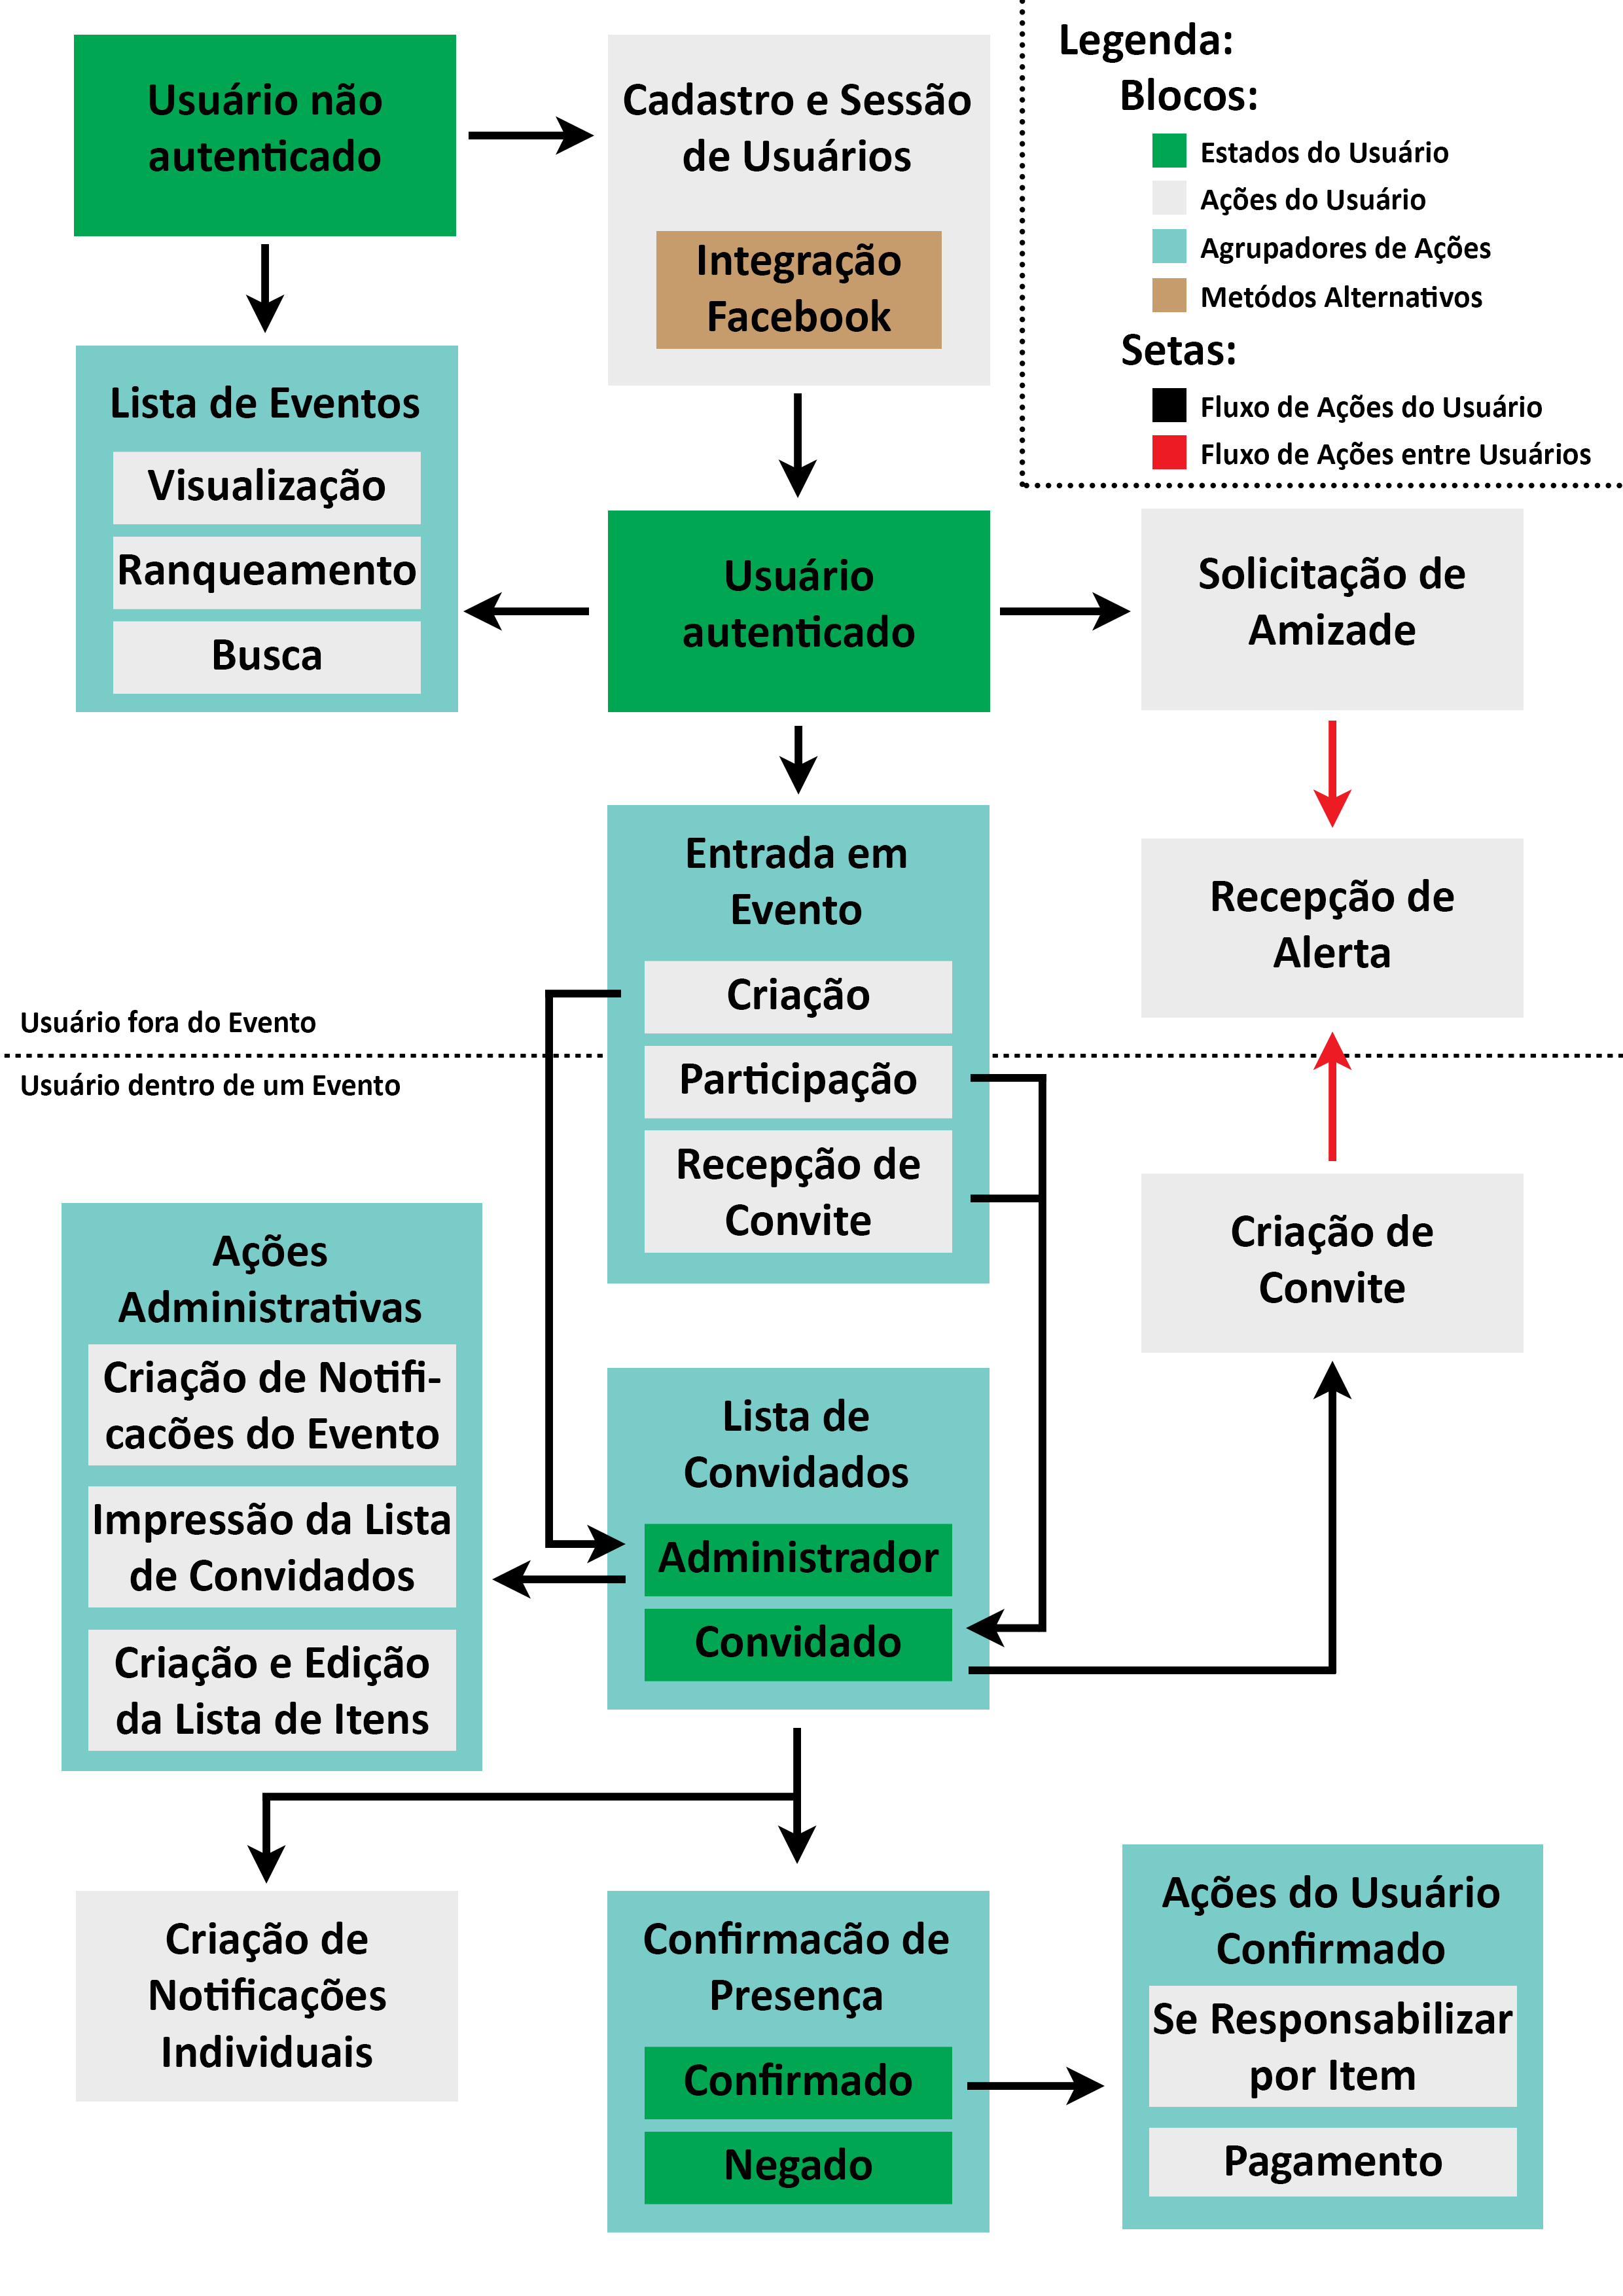
\includegraphics[width=1\textwidth]{figs/esquema_app}
\caption[\textit{Fluxo de ações do usuário no sistema}.]
{Fluxo de ações do usuário no sistema.}
\label{fig:esquemaapp}
\end{figure}

\subsection{Cadastro e Sessão de Usuários}

O projeto tem como objetivo prover funcionalidades aos usuários, tornando-os parte essencial para o bom funcionamento do sistema. Para poder identificá-los e realizar tarefas relacionadas a usuários específicos, é necessário existir sistemas de cadastro e sessão. Basicamente um sistema de cadastro consiste em um formulário que viabiliza a criação de um novo usuário no banco de dados. Um sistema de sessão, por sua vez, permite que ao retornar, esse usuário use um \textit{login} (nome ou e-mail) e uma senha, cadastrados anteriormente, para se identificar.

Por ser um módulo comum em diversos sistemas, existem muitas bibliotecas que tentam facilitar o seu desenvolvimento. No caso do Rails, a gema mais difundida, que também foi utilizada no projeto, se chama Devise~\cite{devise}.

\subsubsection{Devise}

O Devise é uma solução bastante completa para toda a parte de autenticação de usuários. Primeiramente, é muito fácil de ser configurado e é completamente personalizável, garantindo sua popularidade. Vale ressaltar que o recurso gerado pelo Devise (o usuário) é construído seguindo o padrão RESTful, tornando-o ainda mais atrativo. Dentre suas vantagens e funcionalidades estão:

\begin{itemize}
\item Segurança

Senhas criptografadas, com o custo de criptografia personalizável.

\item Histórico

Aliado também à segurança, o Devise já traz informações de data do último acesso, IP de acesso, entre outras.

\item Validação

O e-mail (campo padrão para \textit{login}) e a senha são validados automaticamente.

\item Confirmação por E-mail

Opção que faz com que o usuário receba um e-mail após o início do cadastro, onde o mesmo é finalizado, garantindo que o usuário é, de fato, dono do e-mail.

\item Manter Logado

Módulo que implementa a criação de um cookie no computador do usuário para que sua sessão seja criada automaticamente na próxima vez que retornar ao site.

\item Tempo Limite

O Devise permite o uso de um tempo máximo de inatividade para a sessão, terminando-a automaticamente ao final do prazo.

\item Trancamento de Conta

Outra funcionalidade implementada é a de trancamento de conta, para o caso de muitas tentativas sucessivas mal sucedidas de acesso em sequência. Um e-mail com instruções para destrancar é enviado automaticamente ao e-mail cadastrado, no momento do trancamento.
\end{itemize}

\subsubsection{Filepicker}

Uma parte muitas vezes complicada de sistemas é a utilização de fotos do perfil, sendo necessária a criação de uma parte de upload, hospedagem de arquivos e muitas vezes processamento da imagem como cortes e lógicas para encaixá-la ao layout. Para isso, utilizamos uma ferramenta bastante interessante chamada Filepicker.io~\cite{filepicker}. Todo o processo fica por conta da ferramenta, sendo cobrada uma taxa para tráfegos acima de 5000 fotos/mês. É bastante personalizável e permite além de upload de fotos do próprio computador, acesso a fotos de outros lugares como o Facebook, Google+, Dropbox, entre outros.

\subsection{Integração com Redes Sociais}

Para melhorar ainda mais a experiência do usuário em um sistema web, é muito comum usar contas compartilhadas, evitando que o usuário tenha que lembrar de mais um e-mail e senha. Dessa forma, foi implementada a possibilidade de cadastro e sessão utilizando a conta do Facebook do usuário. Uma gema muito útil e conhecida para isso é o Omniauth-facebook~\cite{omniauth-facebook}, atrelado ao Omniauth~\cite{omniauth}. É necessária a criação de um aplicativo no Facebook Developer (https://developers.facebook.com/) para configurar o Omniauth com uma chave de identificação e senha. Além da utilidade de cadastro e abertura de sessão, o Facebook também provê informações sobre a conta do usuário, mediante autorização, que podem ser úteis na aplicação.
Por ter se tornado popular, até mesmo o Devise implementou uma funcionalidade de integração com o Omniauth, gerando assim uma solução muito robusta e completa.

\subsection{Eventos e Lista de Convidados}

Os eventos são a parte mais importante do projeto, já que tudo gira ao redor deles. Basicamente são instâncias que devem conter informações sobre local, data, hora, preço e privacidade. Além disso, usuários devem ser capazes de criar eventos, confirmar ou negar presença nos mesmos e convidar outros usuários a participarem deles. É importante também a ferramenta de impressão da lista de confirmados para o organizador, de forma a facilitar sua vida no dia do evento.

\subsubsection{Privacidade}
Foram implementados três tipos de privacidade para os eventos:

\begin{itemize}
\item Públicos

Eventos vistos e encontrados por qualquer usuário. Qualquer um pode confirmar presença e convidar pessoas.

\item Privados

Eventos onde somente pessoas convidadas pelo organizador podem ver e confirmar presença, porém, convidados não podem convidar.

\item Convidativos

Parecido com o privado, porém, neste caso os convidados podem convidar mais usuários.
\end{itemize}

\subsubsection{Preço}
O preço do evento depende basicamente de três informações.

\begin{itemize}
\item Preço Fixo

Valor constante, que deve ser pago por todos os confirmados.

\item Preço Compartilhado

Valor constante a ser dividido entre todos os confirmados.

\item Preço de Itens

Valor que representa o somatório dos preços dos itens. Este caso será explicado com mais detalhes na próxima seção.
\end{itemize}

\subsection{Lista de Itens}

Essa funcionalidade é um dos principais diferencias do sistema desenvolvido com relação ao que existe no mercado. Em suma, trata-se de uma lista de itens (como refrigerantes, bola de futebol ou aparelho de som)  que são necessários para a realização do evento. Uma vez criada, usuários podem se tornar responsáveis por itens, isto é, se comprometem a levar o item no dia do evento. Os itens podem ter quantidades específicas, possibilitando que a responsabilidade sobre um mesmo item seja dividida entre mais de um usuário.

Além disso, itens podem possuir preço. Neste caso, o valor somado da lista também será dividido entre os confirmados no evento. O valor de um item, atrelado à quantidade adquirida por um responsável, será descontado do valor a ser pago por este usuário.

\subsection{Pagamento}

Outro diferencial do sistema é a possibilidade de pagamento através do mesmo, dando uma garantia muito maior ao organizador da presença de seus convidados e suporte ao planejamento financeiro do evento. Para que não ocorram problemas, é importante notar que eventos com custo compartilhado ou lista de itens pagos, não poderá ter pagamentos através do sistema, uma vez que, nestes casos, o valor se altera à medida que novos usuários confirmam presença.

O pagamento ocorrerá através do Paypal~\cite{paypal}, uma ferramenta simples e segura de realizar pagamentos na Internet. Eles possuem uma API fácil de utilizar e bastante completa, incluindo até mesmo um ambiente para testes. Sua única desvantagem é que o usuário será redirecionado para um site externo ao sistema na hora de pagar, piorando a experiência do usuário.

O dinheiro irá para a conta do EVNTs, e, após a realização do evento, será transferido para a conta bancária cadastrada pelo usuário. Essa transferência, em um primeiro momento, ocorrerá de forma manual, porém em trabalhos futuros será implementado um sistema automático para isso. Além disso, diversos casos de segurança (principalmente fraudes) ainda não estão sendo contemplados e serão resolvidos também no futuro.

\subsection{Amizades}

Para facilitar a parte de convites para o evento, foi implementado um módulo de amizades, que permite um relacionamento entre dois usuários. Basicamente, um usuário envia uma solicitação de amizade a outro usuário que pode aceitá-la, recusá-la ou até mesmo recusá-la para sempre. Uma vez que a solicitação foi aceita, a amizade é criada. Desta forma, torna-se possível convidar o amigo para eventos de forma simples e direta.

Como já existe a integração com o Facebook no momento do cadastro, a lista de amigos da rede social será aproveitada de forma a automaticamente recriar as amizades dentro do sistema EVNTs, reduzindo o trabalho do usuário.

\subsection{Notificações e Alertas}

Para que o evento não entre no esquecimento, foi implementado um módulo de notificações. A ideia é que o organizador possa criar notificações a serem enviadas para todos os confirmados no seu evento e que cada usuário possa criar notificações individuais para si. Porém, o usuário pode se subscrever ou não às notificações gerais, de forma a evitar casos não desejáveis.

A notificação será na forma de um e-mail que será enviado na data desejada para o usuário indicando a data, horário, local do evento e os itens que aquele usuário deverá levar. Para que ela seja programada para uma data posterior, utilizamos uma gema chamada Delayed Jobs~\cite{delayed_jobs}, que permite de forma bastante simples, executar ações assíncronas no sistema, seja por um sistema de fila, isto é, várias ações para serem executadas em sequência, ou por um sistema de data marcada. Seu funcionamento se dá através de uma tabela no BD onde as ações ficam guardadas e um sistema que verifica a existência de tarefas a serem executadas nessa tabela.

Além disso, há um sistema de alertas para convites de eventos e solicitações de amizades pendentes. Os alertas serão visíveis apenas na aplicação.

\subsection{Ranqueamento de Eventos}

Com o objetivo de divulgar eventos públicos, foi gerado uma lógica para ranqueamento de eventos, com o intuito de, na página inicial do sistema, exibir listas de eventos organizadas de forma interessante ao usuário. Foram implementados dois tipos de listas:

\begin{itemize}
\item Selecionada por distância em relação ao usuário e número de confirmados no evento.

Neste caso, o cálculo da distância é feito através do uso da gema Geocoder~\cite{geocoder}, que permite desde a captura da localização até mesmo o cálculo da distância para um certo ponto geográfico. Utilizamos também a API do Google Maps~\cite{google_maps} que permite visualizações de mapas e um ``auto completar'', utilizado no cadastro de eventos que permite adquirir uma latitude e longitude baseados no endereço.

\item Selecionada pela quantidade de amigos confirmados no evento.
\end{itemize}

Nos dois casos, as listas estarão ordenadas pela data de realização do evento, eliminando eventos ocorridos, proporcionando uma visualização clara e objetiva dos eventos que estão por vir.

\section{Modelos}

Nesta seção, será mostrado em maior detalhe os principais modelos do projeto. Os modelos foram a primeira parte a ser construída do sistema, juntamente com seus testes, já que foi utilizada a metodologia TDD.

Para ajudar no entendimento desta seção, a figura ~\ref{fig:Modelo de Dados - Tabelas e Relacionamentos} pode ser utilizada.

\begin{figure}[H]
\centering
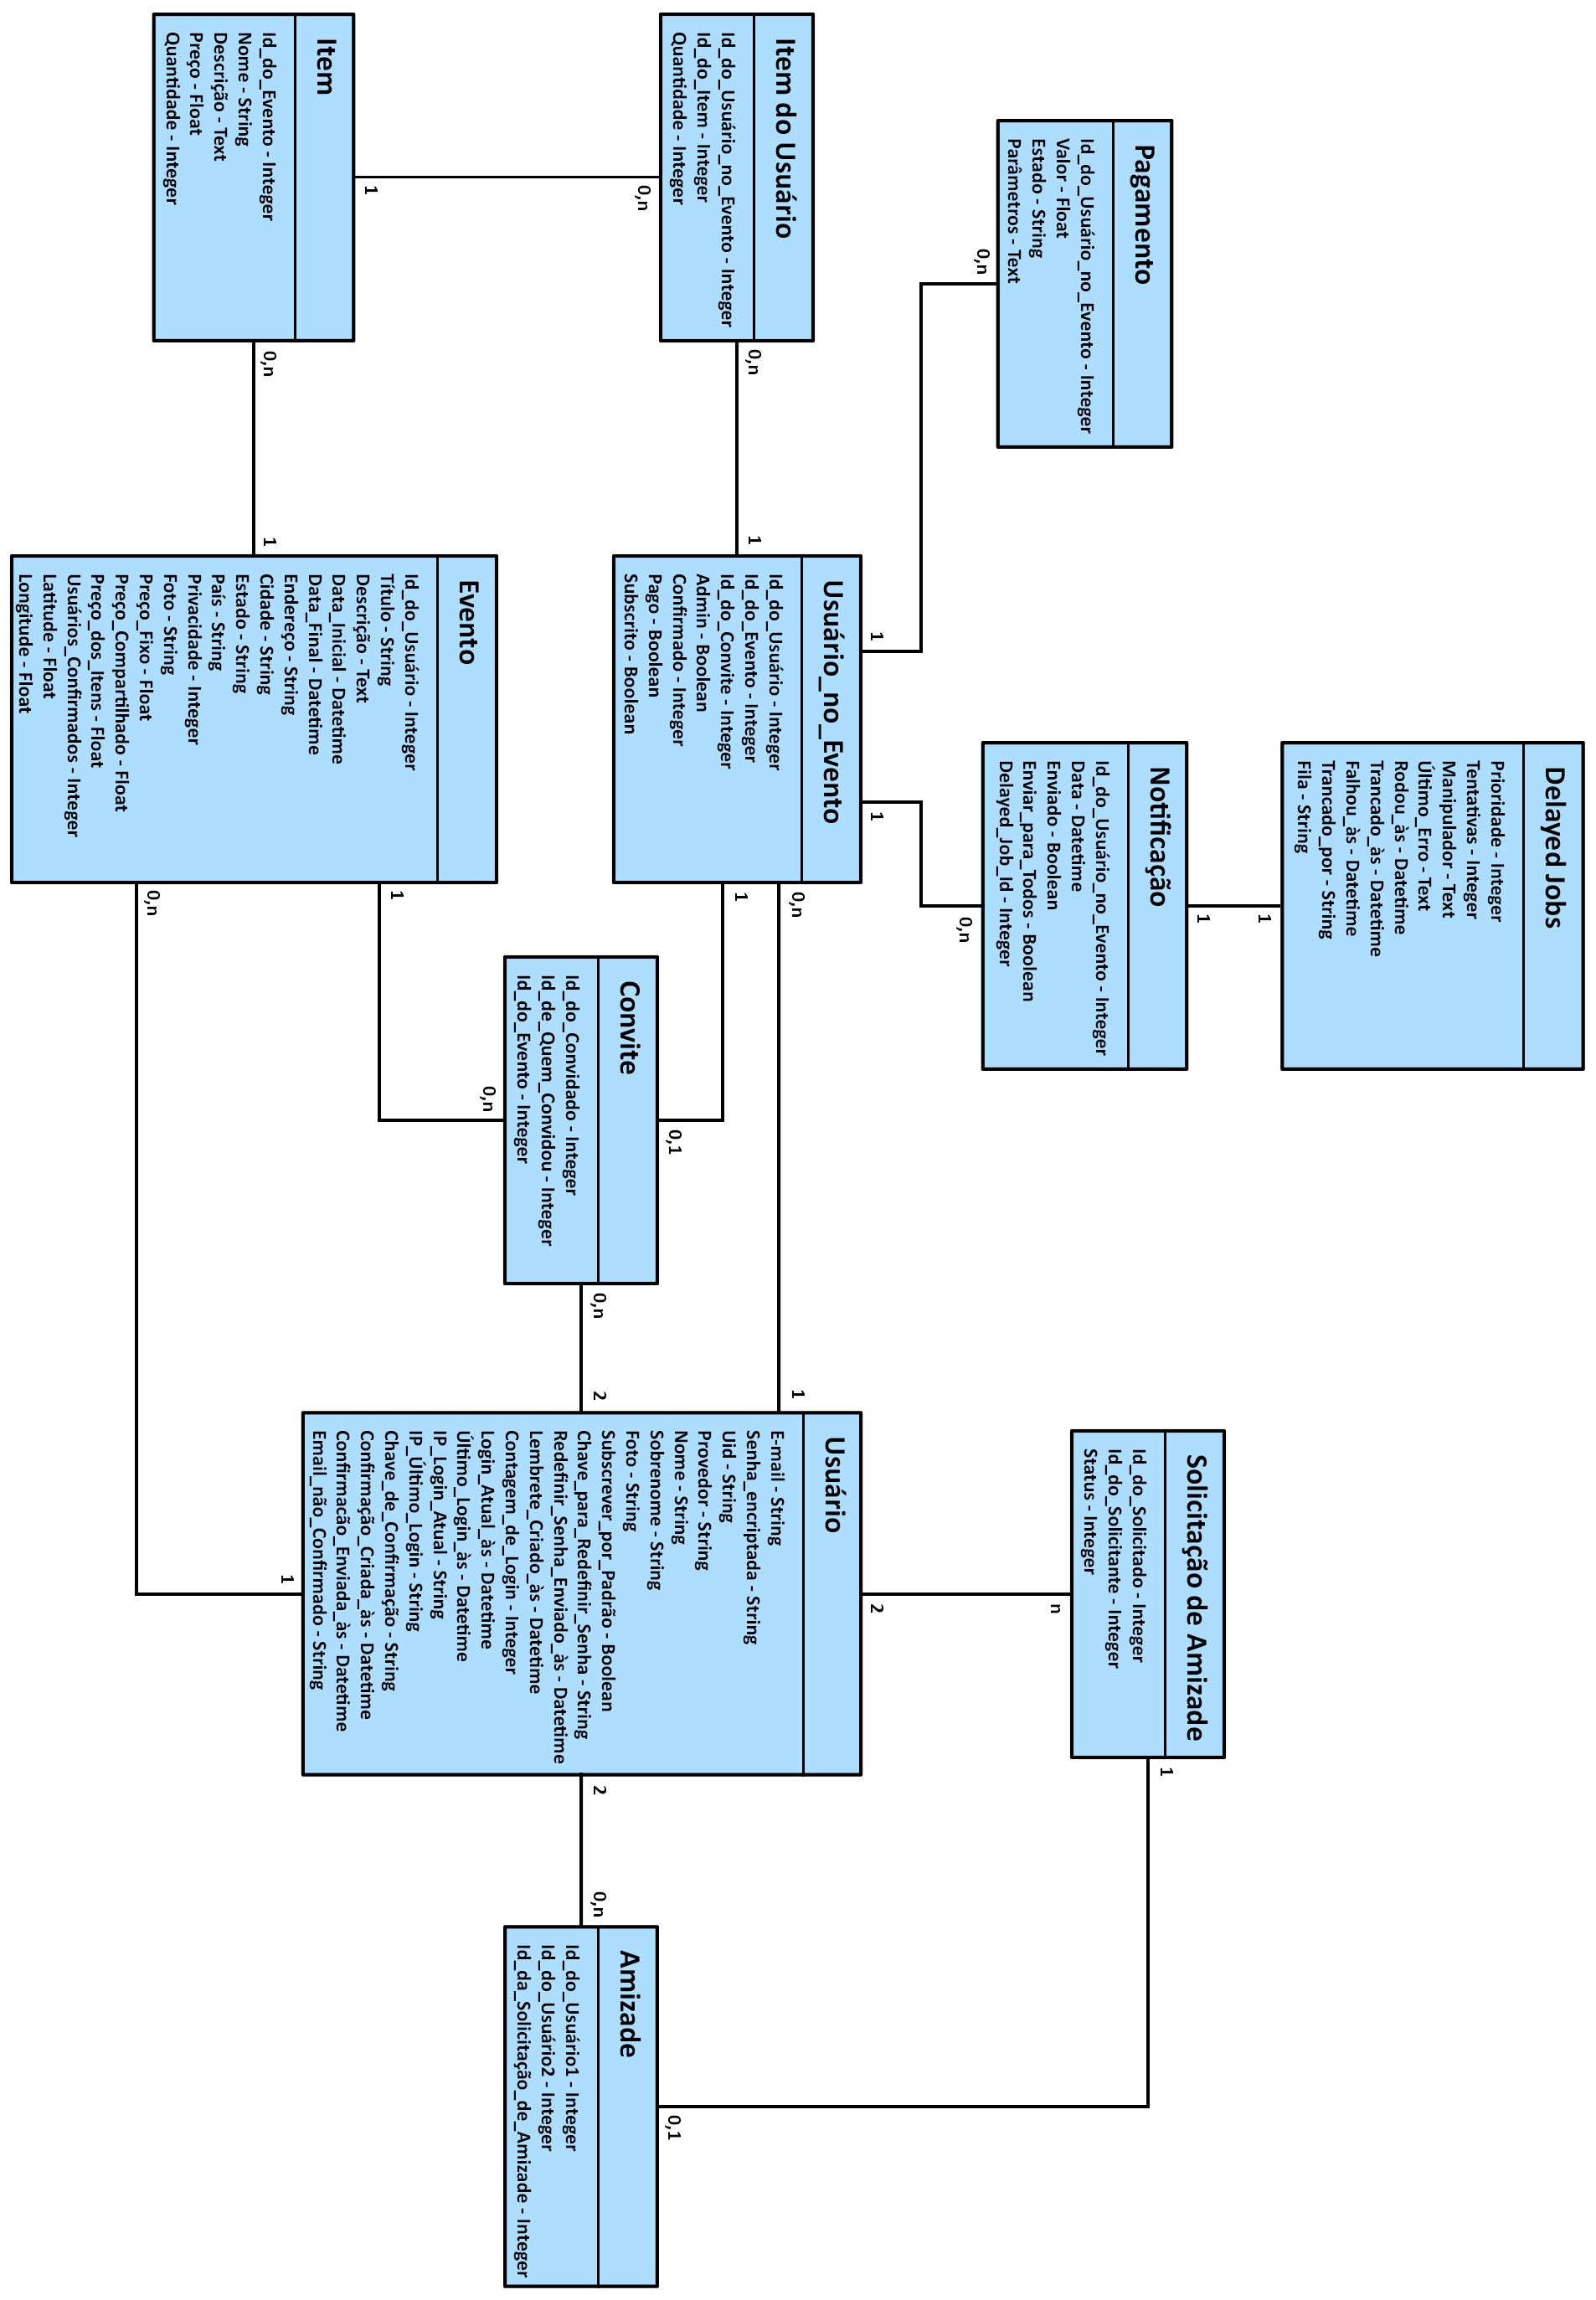
\includegraphics[width=1\textwidth]{figs/modelo_de_dados}
\caption[\textit{Modelo de Dados - Tabelas e Relacionamentos}.]
{Modelo de Dados - Tabelas e Relacionamentos.}
\label{fig:Modelo de Dados - Tabelas e Relacionamentos}
\end{figure}

\subsection{Usuário}

A tabela de usuário possui diversos campos que foram criados devido às funcionalidades do Devise. Primeiramente, o e-mail e senha, já que são os campos padrão do Devise para identificação do usuário. Além disso, por ter sido utilizada a funcionalidade de confirmação por e-mail, os campos \textit{chave\_de\_confirmação}, \textit{confirmação\_criada\_às}, \textit{confirmação\_enviada\_às} e \textit{email\_não\_confirmado} foram criados pela gema. Os campos \textit{contagem\_de\_login}, \textit{login\_atual\_às}, \textit{último\_login\_às}, \textit{ip\_login\_atual} e \textit{ip\_último\_login} são utilizados pela biblioteca para manter o histórico e segurança. Por último, os campos \textit{chave\_para\_redefinir\_senha} e \textit{redefinir\_senha\_enviado\_às} são utilizadas para, com segurança, ter a funcionalidade de ``esqueci minha senha''.

Para o bom funcionamento da integração com o \textit{login} do Facebook, são criados os campos \textit{uid} e o \textit{provedor}. O \textit{provedor} simplesmente guarda por qual provedor estamos fazendo o acesso, para o caso de existir o \textit{login} por outros meios além do Facebook. Já o campo \textit{uid} guarda a identificação do usuário dentro da rede a qual ele pertence.

Os outros campos são bastante intuitivos. O único que vale a atenção é o \textit{subscrever\_por\_padrão}, que tem como objetivo definir se, por padrão, ao entrar num evento o usuário estará subscrito ou não às notificações gerais do mesmo.

\subsection{Evento}

A tabela de eventos é um ponto central do sistema. Como buscas de eventos são bastante comuns, algumas variáveis foram adicionadas à tabela para agilizar esse processo. Entre elas, \textit{cidade}, \textit{estado} e \textit{país} que têm por objetivo restringir os eventos por localidade, \textit{preço\_dos\_itens} e o número de confirmados para evitar o acesso a outras tabelas em funções muito requisitadas e a \textit{latitude} e \textit{longitude}, para rapidamente poder calcular a distância do usuário até o local do evento.

A validação dos campos de eventos é um ponto importante a ser discutido. Como existem tipos de privacidade e de pagamento, é importante que sempre exista a garantia de que esses dados estão consistentes entre si. Além disso, por possuir informações de valores relacionados a outras tabelas, é sempre importante garantir que ao editar um evento, esses valores estejam sempre corretos.

\subsection{Usuário no Evento}

Essa tabela é a terceira tabela essencial para o funcionamento do sistema, já que é ela que relaciona as duas entidades mais importantes (o evento e o usuário). Todas as tabelas que são relacionadas a um usuário no caso dele estar em um evento, se relacionam diretamente com esta tabela, facilitando a implementação de funções relacionadas a esta situação, como um pagamento ou uma notificação.

Além dos campos que identificam seus relacionamentos, essa tabela possui alguns campos importantes:

\begin{itemize}
\item \textit{Admin}

Define se esse usuário tem direitos administrativos sobre o evento, como no caso de ser o organizador.

\item \textit{Confirmado}

Deve ter um valor que indique se o usuário vai, não vai, ou ainda não respondeu se vai ao evento.

\item \textit{Pago}

Evita o acesso a todos os pagamentos (ou tentativas mal sucedidas de pagamento) na hora de saber se usuário já pagou. É importante notar que essa variável possui uma validação importante, já que, além de depender da tabela de pagamentos, é uma parte sensível do fluxo do sistema.

\item \textit{Subscrito}

Define se o usuário receberá as notificações gerais do evento ou não. Vale ressaltar que, por padrão, essa variável assume um valor relativo à variável \textit{subscrever\_por\_padrão} do usuário em questão.
\end{itemize}

\subsection{Notificação}

A tabela de notificação possui algumas singularidades. Primeiramente, o campo \textit{Enviar\_para\_Todos} que é o que diferencia uma notificação geral de um evento para uma notificação personalizada do usuário. É importante notar, que mesmo a notificação geral pertence a um \textit{Usuário\_no\_Evento}, porém, no caso de ser geral, pertencerá ao \textit{Usuário\_no\_Evento} referente ao organizador do evento.

Além disso, para se integrar com a gema Delayed Jobs citada anteriormente, é necessário que exista um campo que relacione a tabela de notificação com um registro na tabela de \textit{Delayed Jobs}. No momento que este registro na tabela de \textit{Delayed Jobs} disparar, ele vai verificar a notificação correspondente e de fato notificar os usuários. Caso o \textit{Enviar\_para\_Todos} seja verdadeiro, essa tarefa irá enviar um e-mail para todos os participantes do evento.

\subsection{Outras Tabelas}

Por serem tabelas mais simples e óbvias, não serão explicitados detalhes. Vale notar que as tabelas \textit{Convite}, \textit{Solicitação\_de\_Amizade} e \textit{Amizade} relacionam dois usuários diferentes entre si. Cada uma com objetivos diferentes.

\subsection{Extras}

Um ponto importante a ser levantado é o relacionamento entre as tabelas. Alguns registros devem ser automaticamente criados a medida que determinadas ações são disparadas. Por exemplo, uma amizade deve ser criada automaticamente quando uma solicitação de amizade é registrada como aceita. Dessa forma, a lógica geral de integração entre os modelos já estará praticamente pronta, deixando para os controladores apenas as ações que de fato ocorrem com a interação de um usuário com o sistema.

\section{Controladores}

Uma vez tendo os modelos prontos e sendo validados, o projeto já está bem encaminhado e então torna-se necessária a criação dos controladores, que recebem as requisições feitas pelos usuários e definem o que deve ser feito. Como citado anteriormente, durante a implementação do projeto usou-se a metodologia RESTful, tornando os controladores bem simples e bem intuitivos, já que quase sempre possuem apenas ações de \textit{Index}, \textit{Show}, \textit{New}, \textit{Create}, \textit{Edit}, \textit{Update} e \textit{Destroy}. Apenas em dois casos essa lógica não se mantém:

\begin{itemize}
\item Busca de evento

Foi criado uma ação especial \textit{Search} para a busca de eventos, deixando o código mais limpo e organizado.

\item Alteração de subscrição

Por ser uma tarefa bem simples e não necessitar de validação por conta do modelo, foi definida uma ação para alterar a subscrição de um usuário às notificações do evento ao invés de usar o método padrão \textit{Update}.
\end{itemize}

Um ponto a ser lembrado é que, por padrão, controladores respondem com HTML, porém em casos de requisições AJAX, essa resposta deve ser dada de forma diferente, seja por um objeto JSON, um XML ou até mesmo Javascript diretamente. Inclusive, é possível configurar um controlador para responder a chamadas diferentes com formatos distintos, ou seja, responder tanto para requisições AJAX quanto a requisições HTTP padrões.

\section{Visões}

Para agilizar o desenvolvimento do \textit{frontend} do sistema, foi utilizado o Bootstrap~\cite{bootstrap}, um \textit{framework} de CSS e Javascript muito intuitivo, de fácil utilização e poderoso. Basicamente, o Bootstrap é um conjunto de classes de estilo (CSS) e funções Javascript a serem utilizadas. Um exemplo de um resultado alcançado rapidamente utilizando bootstrap pode ser observado na figura ~\ref{fig:pagvisuevento}. Trata-se da página de visualização de um evento dentro do sistema implementado. As barras de navegação (no topo e final da página), estilo dos botões, posicionamento em colunas e linhas, campos de preenchimento, entre outros elementos, estão seguindo o padrão do Bootstrap, sendo perceptível o poder da ferramenta e o motivo do seu uso.

\begin{figure}[H]
\centering
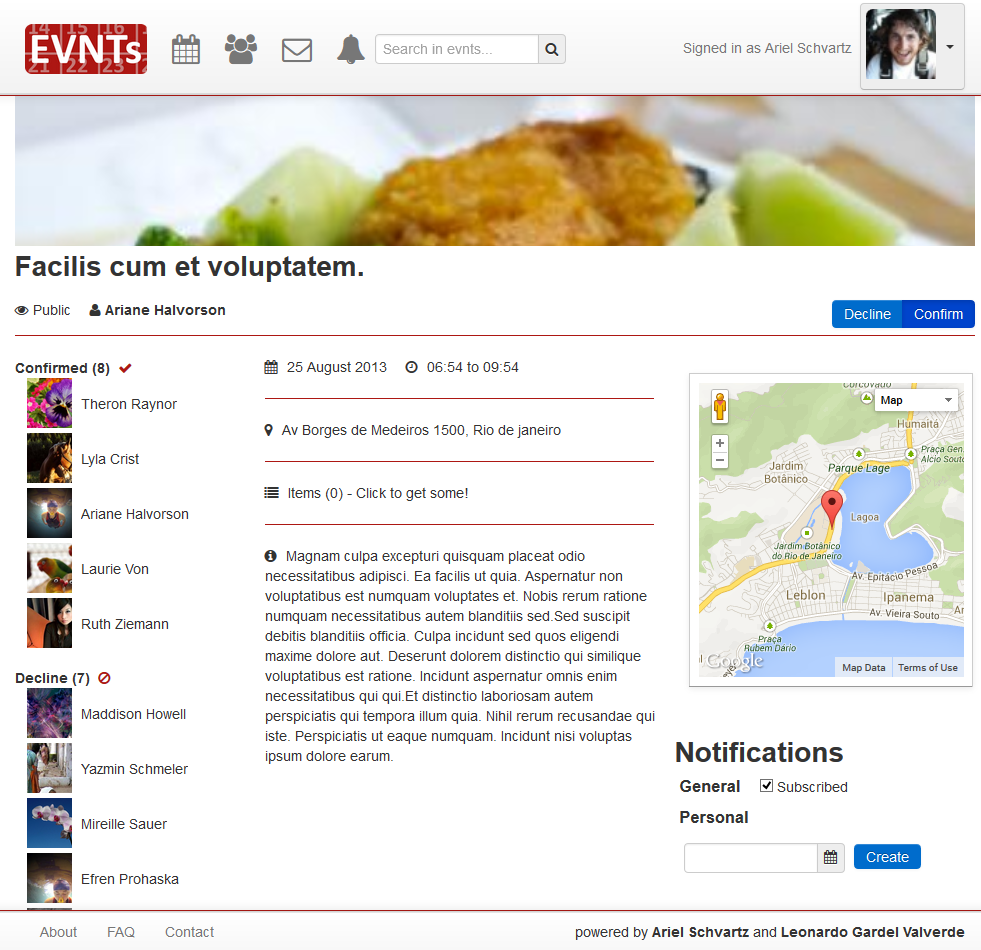
\includegraphics[width=1\textwidth]{figs/event_show}
\caption[\textit{Página de Visualização de Evento}.]
{Página de Visualização de Evento.}
\label{fig:pagvisuevento}
\end{figure}

Além disso, para gerar essa visualização interativa do mapa de localização, foi utilizada a API do Google Maps. Sua utilização é gratuita enquanto o tráfego for pequeno e sua implementação, que se dá através de uma biblioteca em Javascript, é muito fácil e bem documentada.

Outra ferramenta importante para o layout do projeto, foi o Font Awesome~\cite{font_awesome}, que basicamente é biblioteca em CSS que fornece uma fonte que ao invés de conter letras, contém ícones. Dessa forma, os ícones têm qualidade de vetor e são muito leves, já que não são imagens. Seu uso é totalmente gratuito, tornando-o ainda mais atrativo. Ao olhar a figura ~\ref{fig:pagvisuevento}, da página do evento, percebe-se que o uso de ícones torna o site ainda mais agradável e bonito.

Outra questão importante sobre as visões foi o alto uso de AJAX e Javascript. O seu uso evita o carregamento repetidas vezes de páginas completas, reduzindo a quantidade de conteúdo carregado sem necessidade. Dessa forma, obtém-se uma melhora na experiência do usuário, que tem uma resposta mais rápida de suas ações. Outro aspecto bom do uso de Javascript e JQuery é a utilização de animações, criando um sistema mais fluido e agradável. Porém, em contrapartida, usuários podem desativar o Javascript de seus navegadores (principalmente em celulares), apesar de não ser muito comum.

\section{Teste}

Foram implementados testes unitários e funcionais, que representam os testes dos modelos e controladores, como explicado anteriormente.

\subsection{Teste dos Modelos}

Os testes de modelo tem como foco:
\begin{itemize}
\item Validações

Verificar se casos não consistentes de modelos realmente estão sendo validados e negados, enquanto casos consistentes são aceitos pelo sistema. Esses testes garantem registros sempre consistentes no BD.

\item Chamadas de retorno

Diversos modelos devem realizar ações antes ou após serem salvos. Por exemplo, um item, ao ser salvo, deve alterar a variável \textit{Preço\_dos\_Itens} do evento a qual esse item pertence. Neste caso, o valor final da variável deve ser testado para garantir que todas as chamadas estão acontecendo corretamente.

\item Valores padrões

Algumas variáveis devem assumir valores padrões quando o registro é inicializado. Por exemplo, um convite deve gerar um \textit{Usuário\_no\_Evento} com a variável confirmado em um valor padrão para o caso do usuário ainda não ter dado a resposta.
\end{itemize}

Para realizar os testes de modelo e simular dados consistentes e inconsistentes, foram usadas algumas gemas:

\subsubsection{Factory Girl~\cite{factory_girl}}

Permite de forma clara e organizada a criação de registros no banco de dados. Permite a criação de instâncias salvas, não salvas e até mesmo a criação de registros em cadeia, no caso da existência de relacionamentos. A ideia é basicamente criar ``fábricas'' de registros em um arquivo e nos testes apenas chama-las, criando assim um código limpo e DRY (ver seção 2.4)

\subsubsection{FFaker~\cite{ffaker}}

O FFaker, é uma segunda versão da gema Faker, porém reescrita para rodar de forma mais rápida. A ideia da gema é gerar informação básica aleatória, como por exemplo nomes, e-mails, endereços, textos, entre outros. Desta forma, é possível simular informações pseudoaleatórias para testar o sistema.

\subsubsection{Timecop~\cite{timecop}}

Essa gema basicamente permite ``viajar no tempo'' e ``parar no tempo''. Na verdade, o que acontece é que a gema simula horários possibilitando os testes que são dependentes do tempo, como no caso dos testes das notificações. Dessa forma, é possível ``viajar'' até a data onde a notificação deveria ser enviada e verificar se tudo correu bem.

\subsection{Teste dos Controladores}

Os testes dos controladores têm como foco:

\begin{itemize}
\item Rotas e Redirecionamentos

Testes que verificam se as rotas existem e estão retornando sucesso. Além disso, devem verificar que em certos casos, o usuário será redirecionado. Por exemplo, ao criar um evento, o usuário deve ser redirecionado para a página de visualização do evento que acabou de ser criado.

\item Respostas

Testes que avaliam a resposta dada pela rota, isto é, se a requisição foi por AJAX, a resposta não deve ser HTML. Além disso, é importante verificar as informações que são respondidas. Por exemplo, ao criar um novo item por AJAX, deseja-se como retorno o novo item criado, para adicioná-lo à página sem recarregá-la.

\item Permissões

Testes que avaliam casos de permissões de acesso a páginas específicas. Por exemplo, um usuário que não iniciou sua sessão ou que não faz parte de um evento privado não deveria ser capaz de acessar esse evento.

\end{itemize}

Para ajudar nestes testes, além das gemas já mencionadas, foi utilizada a gema Mocha~\cite{mocha}.

\subsubsection{Mocha}

Esta gema permite ``enganar'' o BD, simulando que qualquer instância a ser salva vai ser válida ou não. Isso ajuda muito na hora de testar rotas como o \textit{create} e \textit{update}, simulando casos de sucesso e de falha de forma fácil e rápida.

\section{Ambientes}

Existem três ambientes básicos a serem utilizados pelo sistema. O de desenvolvimento, de testes e de produção. Como o de testes é análogo ao ambiente de desenvolvimento, este não será explicado em detalhes.

\subsection{Desenvolvimento}

Para o ambiente de desenvolvimento, o SGBD utilizado é o SQLite, principalmente por ser muito leve e não precisar de nenhum tipo de configuração para funcionar. Este SGBD se torna suficiente em desenvolvimento, já que a quantidade de dados é baixa e não é necessária uma grande eficiência a nível de BD. Para utilizar o SGBD é necessário instalar a gema referente ao banco.

Neste ambiente, é muito comum o uso do IRB (\textit{Interactive Ruby Shell})
\abbrev{IRB}{\textit{Interactive Ruby Shell}}
, um prompt de comando do seu sistema, onde você pode acessar o BD, chamar funções, entre outros. Seu uso se dá principalmente pela necessidade de depurar o código.

As gemas utilizadas para o ambiente de desenvolvimento foram:

\subsubsection{Pry~\cite{pry}}

O Pry é um substituto do prompt de comando padrão do Rails, o IRB. Suas principais vantagens são a coloração de sintaxe Ruby, a velocidade (rápido comparado ao IRB) e a possibilidade de invoca-lo em tempo de execução. Esta última funcionalidade se torna extremamente necessária e importante para depurar código, já que a qualquer momento do fluxo de execução é possível travar o sistema e ter comandos Ruby a sua disposição.

\subsubsection{Letter Opener~\cite{letter_opener}}

Essa gema permite visualizar diretamente no browser, um e-mail que seria enviado. Isso evita a necessidade de configurar uma conta de e-mail no ambiente de desenvolvimento. Além de agilizar o processo de configuração do sistema e de visualização dos e-mails, a gema ainda evita que diversos e-mails sejam mandados para sua caixa de entrada.

\subsubsection{Better Errors}

Essa gema faz um trabalho bastante simples mas que ajuda muito na depuração de erros. Basicamente, a ideia é melhorar as páginas de erros. Ao invés de simplesmente uma mensagem jogada na tela, outras informações como inspeção de variáveis também são mostradas e a visualização do erro é muito mais agradável e de fácil leitura.

\subsection{Produção}

Para produção, utilizamos o Heroku~\cite{heroku}, uma plataforma de aplicativos na nuvem que permite aos desenvolvedores se focarem somente no desenvolvimento de código, sem ter de se preocupar com gerenciamento de servidores, implantação ou escala. Além disso, existe um plano gratuito, obviamente limitado, porém completo e bastante útil para testar com usuários reais em um primeiro momento. Para garantir a facilidade no momento de implantação, esta se dá através do próprio GIT se tornando rápida e fácil.

Por padrão, o Heroku usa como SGBD o Postgres, que é um banco de dados robusto e eficiente quando comparado a outros SGBDs. Portanto, foi instalada a gema do Postgres para se adequar aos requisitos do sistema.

  \chapter{Modelo de Negócios}

O modelo de negócios de uma empresa basicamente define onde uma empresa executa e vende seus produtos e (ou) serviços. Além disso, deve mostrar o valor que o produto (ou serviço) oferece para os seus clientes, definindo de que forma a empresa lucrará ao entregar esse valor para seus consumidores. Em outra palavras, a empresa irá definir o que fazer, porque fazer e como fazer, traçando uma linha de objetivos e caminhos a serem seguidos pela empresa. O modelo é útil tanto para empresas grandes que precisam reduzir custos, redefinir estratégias, entre outros, quanto para empresas iniciantes, que precisam definir suas diretrizes e, muitas vezes, de um grande documento que apresente os recursos necessários para dar início à empresa~\cite{modelo_de_negocios}.

Existem alguns métodos para se definir um modelo de negócios, sendo que em sua maioria, são técnicas complementares. A mais conservadora é a criação de um plano de negócios, técnica muito difundida e utilizada. Porém, nos dias de hoje, uma outra técnica vem ganhando muito espaço, o BMC (\textit{Business Model Canvas}).
\abbrev{BMC}{Business Model Canvas}
A seguir serão apresentadas vantagens e desvantagens de cada um destes métodos, visando permitir uma melhor análise comparativa entre eles~\cite{comparabmcplanoum}~\cite{comparabmcplanodois}.

\section{Plano de Negócios}

O plano de negócios tem como objetivo especificar em detalhes o negócio que está sendo analisado. Por esse motivo, ao final do processo é gerado um documento muito extenso e explicativo relativo a todas as áreas da empresa. Além de uma explicação detalhada da empresa, seus objetivos e propostas de valor, sua produção pressupõe a criação de um plano financeiro, plano de marketing, plano de recursos humanos e um cronograma completo.

\subsection{Vantagens}

\begin{itemize}
\item Facilidade na aquisição de investimentos para o negócio, já que, além de mais detalhes, apresenta um plano financeiro, explicitando gastos e previsões sobre o tempo de retorno.
\item Ajuda a prever todas as áreas da empresa, tendo uma visão macro do negócio e aumentando o entendimento dos sócios em cada área.
\end{itemize}

\subsection{Desvantagens}

\begin{itemize}
\item É um processo muito demorado e requer muita pesquisa. Pode demorar semanas ou até meses para ser criado.
\item Muitas vezes, os sócios ainda não têm conhecimento sobre algumas hipóteses, podendo levar à criação de um plano inconsistente e irreal.
\item Diversas variáveis mudam com o tempo e são imprevisíveis, de forma que o plano pode se desatualizar rapidamente.
\item Os sócios, em geral, acabam utilizando informações incorretas ou não embasadas em diversos pontos do plano, gerando um documento muitas vezes inconsistente.
\item Se ocorre uma mudança na empresa, é necessário mudar todo o plano, tendo um custo de atualização altíssimo.
\end{itemize}

\section{BMC}

Inicialmente proposto por Alexander Osterwalder, o BMC visa produzir o modelo de negócios rapidamente e de forma dinâmica. O documento final é de apenas uma folha pré-formatada com nove blocos que definem o modelo de negócios. São eles: principais atividades, principais recursos, rede de parceiros, proposição de valor, segmentos de clientes, canais, relacionamento com o cliente, estrutura de custos e fluxos de receita. A ideia sugere a utilização de \textit{post-its} para que definições possam ser alteradas com facilidade.~\cite{tutorialbmc}

\subsection{Vantagens}

\begin{itemize}
\item Velocidade de produção, já que contém apenas uma folha com um padrão claro de preenchimento.
\item Modelo preparado para mudanças ao longo do processo, considerando que um empreendedor nem sempre já tem de início o conhecimento necessário na área onde estará atuando.
\item Cria um documento enxuto, isto é, focado apenas no que é mais importante, evitando perda de tempo com detalhes que têm grandes chances de serem alterados.
\item Por estar sempre sendo revisado, propicia a inovação e melhoria das ideias sobre a empresa.
\end{itemize}

\subsection{Desvantagens}

\begin{itemize}
\item Por ser um documento de criação simples e rápida, muito vezes acaba sendo superficial.
\item Pode conter dados inconsistentes, visto que os criadores nem sempre estudam e pesquisam a respeito da área de atuação.
\item Ainda não é visto por investidores como um substituto do plano de negócios, tornando necessário o desenvolvimento do plano mais completo na hora de angariar recursos.
\end{itemize}

\section{Blocos do BMC}

\subsection{Principais Atividades}

Este bloco visa definir todas as atividades que são necessárias para executar o modelo de negócios da empresa. Basicamente, estas atividades fazem com que todas as informações descritas nos outros blocos sejam alcançadas.

\subsection{Principais Recursos}

Esta área do documento tem como objetivo explicitar todos os recursos necessários para entregar o devido valor para seus clientes e ter uma renda em cima disso. Os itens dessa seção devem incluir recursos tangíveis e até mesmo os intangíveis. Em geral existem quatro categorias de recursos:

\begin{itemize}
\item Recursos Físicos

Envolvem máquinas, escritórios, instalações, entre outros.

\item Recursos Intelectuais

Neste são consideradas marcas, patentes ou informações (em um BD, por exemplo). Apesar da dificuldade de se gerar recursos intelectuais, uma vez gerados, são muito valiosos.

\item Recursos Humanos

Como o próprio nome já diz, visa definir os empregados necessários para o funcionamento da empresa.

\item Recursos Financeiros

Definem valores como investimentos ou linhas de crédito, necessários para tirar a empresa do papel e colocá-la para funcionar.
\end{itemize} 

\subsection{Rede de Parceiros}

A rede de parceiros tem como objetivo definir quem são fornecedores e parceiros que fazem o modelo funcionar melhor. Isso pode envolver possíveis parcerias com não-concorrentes, concorrentes, fornecedores e compradores. Como motivação para as parcerias, pode-se considerar:

\begin{itemize}
\item Otmização e escala devido à melhor alocação de recursos e redução de custos.
\item Para tentar minimizar o risco e as incertezas do projeto, é comum a parceria entre empresas concorrentes.
\item Ao invés de desenvolver novas atividades na empresa, muitas vezes é melhor focar no que se sabe fazer, e criar uma parceria com quem o complemente. Então, ao criar parcerias, estendem-se a capacidade e as atividades da empresa.
\end{itemize}

\subsection{Proposição de Valor}

Esta seção é alma do documento. Nela está descrita a proposta de valor entregue ao cliente através do produto, ou seja, é o valor observado pelo cliente no produto ou serviço oferecido. Consequentemente, é determinante na aquisição de novos clientes. Diversos elementos podem contribuir à proposta de valor, como: inovação, design, preço, usabilidade, entre outros.

\subsection{Segmentos de Clientes}

Essa área visa definir quem são os consumidores e clientes da empresa. Numa situação de um crescimento muito grande da base de clientes, se torna interessante dividí-los em segmentos de forma a atendê-los melhor. Os segmentos podem ser de massa (não há distinção de clientes), de nicho (focado em uma área de atuação), diversificados (que atendem diversas áreas) ou até mesmo mercados multilaterais (que trabalham com mais de um segmentos para funcionar).

\subsection{Canais}

Como o próprio nome já diz, visa definir os canais de comunicação, distribuição e venda do produto ou serviço. Eles são muito importantes para saber com clareza por onde o consumidor irá conhecer o produto, onde irá adquirí-lo e por onde poderá dar um feedback. É importante avaliar por onde aumentar a base de clientes, como de fato passar a proposta de valor ao cliente, como entregar esse valor e como dar suporte ao consumidor. Dessa forma, todo o canal de comunicação estará definido.

\subsection{Relacionamento com o Cliente}

Este bloco define que tipo de relacionamento com o cliente ocorrerá. Existem diversas possibilidades, como uma assistência pessoal, comunidades (consumidores se ajudam) ou até mesmo por meio de auto ajuda, onde a empresa oferece meios ao consumidor para descobrir sozinho o que precisa.

\subsection{Estrutura de Custos}

Esta parte do BMC tenta definir quais são os gastos necessários para o bom funcionamento da empresa. Além disso, tenta encontrar recursos e atividades que são muito caros. Se o resto do documento já estiver preenchido, se torna mais fácil definir a estrutura de custos. Basicamente, existe em empresas focadas em reduzir custos e empresas focadas em agregar valor ao seu produto ou serviço. As duas formas visam aumentar o lucro, porém de maneira oposta.

É importante também dar o devido valor ao tipo de custo, isto é, se é um custo fixo, onde os custos se mantém ao longo do tempo, ou variável, que variam de acordo com o volume de produto ou serviço.

\subsection{Fluxos de Receita}

Fluxos de receita definem a renda gerada por cada segmento de clientes, definindo quanto cada um deles está disposto a pagar pela proposta de valor. As fontes de receita podem ser geradas de diversas formas, desde uma venda específica, venda de assinaturas, venda de anúncios ou até mesmo licenciando o produto ou serviço da empresa.

\section{Modelo de Negócios do EVNTs}

Neste capítulo, será apresentado o modelo de negócios do projeto. Primeiramente, analisando as vantagens e desvantagens, foi escolhido aplicar o BMC, já que o trabalho é focado em desenvolvimento ágil. Além disso, o BMC é interessante por facilitar modificações futuras, que certamente ocorrerão. O BMC produzido pode ser visualizado na ~\ref{fig:bmc}.

\begin{figure}[H]
\centering
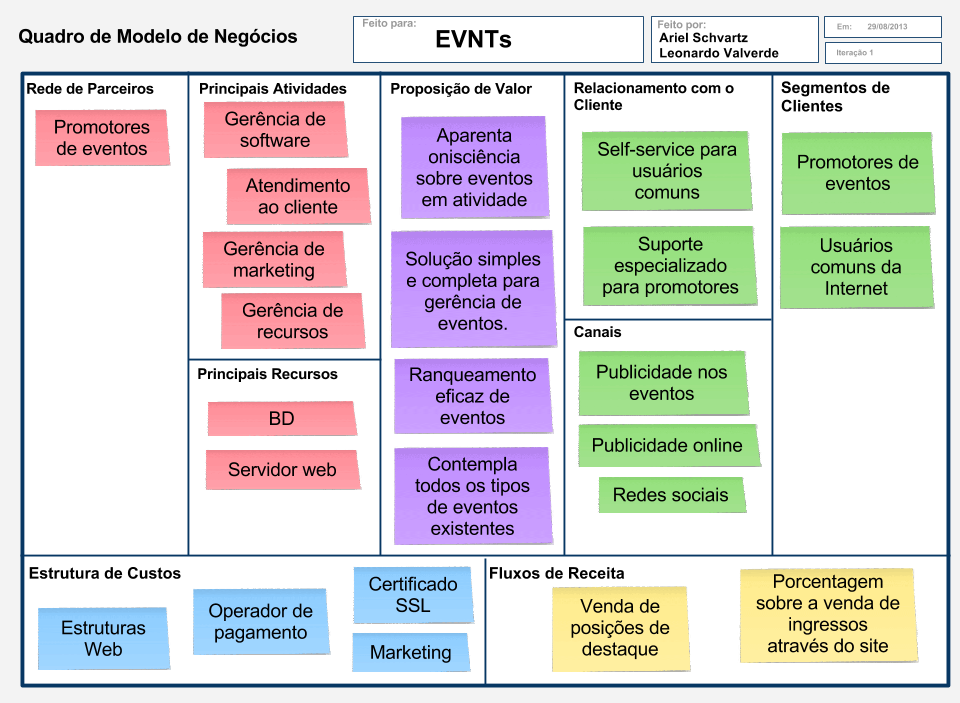
\includegraphics[width=1\textwidth]{figs/bmc}
\caption[\textit{BMC do projeto}]
{BMC do projeto}
\label{fig:bmc}
\end{figure}

Como o BMC é uma representação muito sucinta do negócio, será realizado a seguir um detalhamento de cada tópico incluído no mesmo.

\begin{itemize}

\item Proposições de Valor

\begin{itemize}

\item Aparenta onisciência sobre os eventos em atividade

Obviamente, é essencial para o sucesso da aplicação que nela estejam cadastrados muitos eventos. De forma ideal, pode-se imaginar o caso extremo, onde todos os eventos existentes estão mapeados na aplicação.

\item Ranqueamento eficaz de eventos

De nada adianta mapear boa parte dos eventos existentes sem um ranqueamento eficiente. É humanamente impossível detectar eventos interessantes dentre uma lista não ordenada contendo todos os eventos em atividade. A ferramenta de ranqueamento é vital para o sucesso da aplicação.

\item Contempla todos os tipos de eventos existentes

Como citado anteriormente, uma das grandes deficiências dos sistemas vigentes que auxiliam na gerência de eventos é a sua pouca versatilidade. A aplicação deve dar suporte aos diferentes tipos de eventos existentes, de forma a permitir manutebilidade ao seu gerenciamento.

\item Solução simples e completa para a gerência de eventos

Um dos principais focos é oferecer todas as ferramentas demandadas pelo usuário, no que diz respeito à gerência de eventos. A ideia é que os usuários não precisem utilizar nenhuma outra plataforma para realizar tal tarefa.

\end{itemize}

\item Principais Recursos

\begin{itemize}

\item Banco de Dados

O Banco de Dados é um recurso essencial para o funcionamento do sistema. Além disso, é responsável pelo armazenamento de informações, sendo um recurso intelectual de extrema importância.
\item Servidor Web

Além do BD, o servidor é o outro pilar essencial para que um sistema web funcione plenamente. Dessa forma, se torna outro recurso essencial para o modelo de negócios. Sua escolha afeta a manutenção, custo e escalabilidade do projeto.
\end{itemize}

\item{Segmentos de Clientes}

\begin{itemize}
\item Usuários Comuns da Internet

O aplicativo foca em prover funcionalidades úteis a qualquer pessoa. Ou seja, em um primeiro momento, qualquer um que esteja conectado à Internet poderá se interessar por usar o EVNTs, caracterizando-se assim, um segmento de massa.

\item Promotores de Eventos

Os promotores de eventos são usuários organizadores de grandes eventos públicos e pagos, sendo assim extremamente valiosos para o projeto. Dessa forma, são os usuários que, provavelmente, criarão os eventos com a maior quantidade de pessoas confirmadas dentro do sistema. Assim, além de serem grandes geradores de renda (ver a parte de fluxos de receita) serão atrativos para novos usuários.
\end{itemize}

\item{Rede de Parceiros}

\begin{itemize}
\item Promotores de Eventos

Além de usuários do sistema, organizando eventos, os promotores podem ser considerados também parceiros. São pessoas de suma importância para a criação de uma grande base de eventos, pois através de uma relação de benefício mútuo, os promotores encontram no sistema um local para divulgação e venda de ingressos, enquanto atraem novos clientes a este.
\end{itemize}

\item{Canais}

\begin{itemize}
\item Publicidade nos Eventos

Este canal visa fazer um contato \textit{offline} com os clientes. A ideia é que em grandes festas, shows e outros eventos públicos, sejam colocadas propagandas (como cartazes e banners) de forma a mostrar aos usuários, por exemplo, que poderiam ter adquirido ingressos por meio da aplicação.

\item Publicidade \textit{Online}

Uma das formas mais utilizadas para divulgação de aplicativos web é a realização desta por meio de propagandas em sites. É um método extremamente eficiente, pois basta um clique para que o usuário acesse o sistema. Existem empresas muito populares que proveem este serviço, proporcionando ao contratante um grau de visibilidade proporcional ao pagamento realizado.

\item Redes Sociais

As redes sociais vêm cada vez mais se tornando o principal meio de divulgação para micro e pequenas empresas, já que são baratas (ou até mesmo gratuitas) e, com dedicação, é possível uma boa alcançabilidade. 

\end{itemize}

\item{Relacionamento com o Cliente}

\begin{itemize}
\item Auto ajuda para usuários comuns

Em geral, como teremos uma gama muito grande de usuários, torna-se muito custosa a criação de um sistema de suporte pessoal. Porém, por dispor de diversas funcionalidades inéditas pelos usuários, é importante que se estabeleça um relacionamento através de um sistema auto ajuda, como um FAQ (\textit{Frequently Asked Questions})
~\abbrev{FAQ}{\textit{Frequently Asked Questions}}
para auxiliá-los.

\item Suporte Especializado para Promotores

Por terem uma importância muito grande para o sistema, é essencial oferecer atendimento especial aos promotores, além de suporte personalizado, de forma a deixá-los a vontade com o sistema e sem dúvidas sobre o funcionamento do mesmo.

\end{itemize}

\item{Principais atividades}

\begin{itemize}
\item Gerência de \textit{Software}

Se faz necessária uma equipe de desenvolvimento e manutenção do \textit{software}, para garantir o seu bom funcionamento, além de proporcionar melhorias ao mesmo.

\item Atendimento ao Cliente

É necessária uma equipe voltada para o relacionamento com os clientes, citado anteriormente. Isso inclui esforços tanto para a manutenção do sistema de auto ajuda como para o contato direto com os promotores.

\item Gerência de Marketing

Equipe especializada em estudar locais (\textit{online} e \textit{offline}) para divulgação do sistema, além de criar campanhas nos mesmos, inclusive em redes sociais.

\item Gerência de Recursos

É essencial que o caixa da empresa seja gerenciado de forma inteligente. Para isso é necessário que haja uma equipe voltada para a gerência de recursos do projeto, distribuindo-os ao longo dos demais setores da empresa.

\end{itemize}

\item{Fluxos de Receita}

\begin{itemize}

\item Porcentagem sobre a Venda de Ingressos

A principal fonte de receita da empresa, se baseia na venda de ingressos. Basicamente, seria cobrado um percentual do valor do ingresso pelos serviços sendo prestados. O organizador, pode optar por incluir esse valor ao preço do ingresso ou deixar que o usuário pague por ele.

\item Venda de Posições de Destaque

Outra forma de gerar receita, seria através da venda de posições de destaque para eventos. Com isso, haveria uma área no site de ``Eventos em Destaque'' com os eventos que pagaram para ter aquela posição especial.

\end{itemize}

\item{Estrutura de Custos}

\begin{itemize}

\item Estruturas Web

Os gastos em estruturas web basicamente são representados com: servidor, banco de dados e domínio.

\item Operador de Pagamento

O operador de pagamento, em um primeiro momento, será o PayPal por seu selo de segurança e praticidade de implementação. Porém, é um custo muito alto para a empresa, já que o valor cobrado é de 5,4\% a 6,4\% + R\$0,60 por transação. É importante ter em mente que se faz necessária a pesquisa por outras soluções de pagamento, para não inviabilizar o projeto.

\item Certificado SSL

Como explicado na parte de segurança do Rails, é importante o uso de conexões SSL, para que informações se tornem criptografadas e, consequentemente, seguras. Para que o usuário saiba que um site é criptografado, existem empresas que vendem certificados SSL, atestando a segurança do mesmo.

\item Marketing

Marketing é um dos principais gastos de qualquer empresa que quer crescer rapidamente. Além dos gastos com uma equipe, existem diversos outros relacionados aos meios de divulgação e a produção de campanhas.

\end{itemize}

\end{itemize}

  \chapter{Conclusão e Trabalhos Futuros}

\section{Conclusão}

O \textit{framework} Ruby on Rails proporcionou o desenvolvimento da aplicação de forma extremamente ágil. O tempo para produção desta poderia ser ainda mais reduzido, caso não fosse preciso um tempo de aprendizado para utilização de diversas ferramentas e metodologias. Porém, vale ressaltar que ambos os programadores do projeto possuíam razoável experiência na utilização deste \textit{framework}, tendo passado por um processo de aprendizado relativamente longo. Desta forma, este projeto razoavelmente complexo pôde ser produzido em um número reduzido de horas de trabalho.

Técnicas como o TDD contribuíram enormemente para a produção de um código claro e manutenível, por todas as razões elucidadas anteriormente. Foi percebida uma dificuldade inicial na adoção deste método, já que os desenvolvedores não estavam habituados à realização de testes de forma precoce. Entretanto, a sua utilização proporcionou uma experiência positiva, deixando claras as vantagens da utilização desta técnica.

Ao longo do curso de graduação, foi introduzido apenas o conceito de plano de negócio. Porém, após pesquisas, foi descoberto que o BMC é uma técnica mais atual e interessante para empresas iniciantes. O seu aprendizado e realização foi uma experiência extremamente valiosa, pois possibilita o empreendimento de forma ágil.

Pode-se concluir através dos resultados demonstrados pelo BMC que o projeto possui um bom potencial de rentabilidade. Desta forma, pretende-se dar continuidade a este empreendimento visando torná-lo público em breve. Entretanto, para que isso seja possível se fazem necessários alguns ajustes, que serão enumerados na seção a seguir.

\section{Trabalhos Futuros}

\subsection{Pagamento}

A funcionalidade de pagamento do sistema, apesar de implementada, não está otimizada, sendo necessárias melhorias:

\begin{itemize}
\item Transferência Automática de Verba para Organizadores

Como citado anteriormente, um gargalo para a escalabilidade do projeto é a necessidade de transferência manual de verbas para os organizadores dos eventos. Devido à dificuldade de implementação, esta característica foi deixada para o futuro.

\item Fraudes

Existe uma série de pontos de falha que deve ser cuidadosamente coberta. Um deles consiste na criação de eventos falsos com a finalidade de angariar fundos dos usuários por meio da funcionalidade de pagamento. A princípio, este problema pode ser sanado através de uma verificação presencial a respeito da existência do evento, porém, este método prejudica enormemente a escalabilidade do projeto. Diversas possíveis soluções foram pensadas para evitar estes e outros tipos de fraudes, porém todas possuem brechas, sendo necessária uma análise de risco mais aprofundada.

\item Sistema Próprio de Pagamento

A utilização de sistemas de pagamento terceirizados (como o PayPal) são muito custosos ao empreendimento. A complexidade da implementação de um sistema de pagamentos “online” inviabilizou a sua execução até o momento, porém, é sabido que este é um ponto chave para o sucesso do projeto.

\end{itemize}

\subsection{Segurança}

A aplicação ainda possui diversas brechas de segurança, que precisam ser identificadas e combatidas. É necessário um longo trabalho de aprimoramento até que tenhamos uma versão de fato segura.

\subsection{Parcerias e Sociedade}
\begin{itemize}

\item Promotores

Como já dito anteriormente, as parcerias ajudam no alavancamento do site. Então, para um crescimento acelerado, um dos próximos passos seria a busca por promotores interessados.

\item Designers

Uma parte que ainda está precária no sistema devido à falta de conhecimento por parte dos desenvolvedores, é a parte de design. Dessa forma, torna-se importante a parceria ou sociedade com algum designer ou empresa do ramo, visando a produção de um resultado ainda melhor.

\item Investidores

Outro foco que deve ser dado aos trabalhos futuros, é a busca por recursos financeiros, já que, apesar de baixos, o empreendimento tem custos que precisam ser sanados. Além disso, seria interessante que os criadores pudessem dar atenção total ao projeto, sendo necessário um salário para mantê-los.

\end{itemize}

Além destas, também são necessárias outras parcerias, como para gerência administrativa e de marketing do projeto. Porém estas só são necessárias em uma fase mais avançada do empreendimento, já que inicialmente não existe fluxo de caixa que torne-as indispensáveis.

  \backmatter
  \bibliographystyle{coppetex/coppe-unsrt}
  \bibliography{projeto}
\end{document}